\documentclass[oneside,numbers,spanish]{ezthesis}
%% # Opciones disponibles para el documento #
%%
%% Las opciones con un (*) son las opciones predeterminadas.
%%
%% Modo de compilar:
%%   draft            - borrador con marcas de fecha y sin im'agenes
%%   draftmarks       - borrador con marcas de fecha y con im'agenes
%%   final (*)        - version final de la tesis
%%
%% Tama'no de papel:
%%   letterpaper (*)  - tama'no carta (Am'erica)
%%   a4paper          - tama'no A4    (Europa)
%%
%% Formato de impresi'on:
%%   oneside          - hojas impresas por un solo lado
%%   twoside (*)      - hijas impresas por ambos lados
%%
%% Tama'no de letra:
%%   10pt, 11pt, o 12pt (*)
%%
%% Espaciado entre renglones:
%%   singlespace      - espacio sencillo
%%   onehalfspace (*) - espacio de 1.5
%%   doublespace      - a doble espacio
%%
%% Formato de las referencias bibliogr'aficas:
%%   numbers          - numeradas, p.e. [1]
%%   authoryear (*)   - por autor y a'no, p.e. (Newton, 1997)
%%
%% Opciones adicionales:
%%   spanish         - tesis escrita en espa'nol
%%
%% Desactivar opciones especiales:
%%   nobibtoc   - no incluir la bibiolgraf'ia en el 'Indice general
%%   nofancyhdr - no incluir "fancyhdr" para producir los encabezados
%%   nocolors   - no incluir "xcolor" para producir ligas con colores
%%   nographicx - no incluir "graphicx" para insertar gr'aficos
%%   nonatbib   - no incluir "natbib" para administrar la bibliograf'ia

%% Paquetes adicionales requeridos se pueden agregar tambi'en aqu'i.
%% Por ejemplo:
%\usepackage{subfig}
%\usepackage{multirow}

%% # Datos del documento #
%% Nota que los acentos se deben escribir: \'a, \'e, \'i, etc.
%% La letra n con tilde es: \~n.


\usepackage{titlesec}
\usepackage{fancyhdr}
\usepackage[Sonny]{fncychap} %Options: Sonny, Lenny, Glenn, Conny, Rejne
                             %         Bjarne, Bjornstrup
\usepackage{lmodern}
\usepackage{listings}
\usepackage{color}
\usepackage{array}
\usepackage{colortbl}
\usepackage{url}
\usepackage{xcolor}
\usepackage[utf8]{inputenc}
\usepackage{caption}
\usepackage{float}


\setcounter{secnumdepth}{4}

\author{Carlos Alberto Llano Rodríguez}
\title{VirtShell - Framework para aprovisionamiento de soluciones virtuales}
\degree{Maestría en Ingeniería con énfasis en Ingeniería de Sistemas}
\supervisor{Jhon Alexander Sanabria}
\institution{Universidad del Valle}
\faculty{Escuela de Ingeniería de Sistemas y Computación}
\department{Facultad de Ingeniería}

%% # M'argenes del documento #
%% 
%% Quitar el comentario en la siguiente linea para austar los m'argenes del
%% documento. Leer la documentaci'on de "geometry" para m'as informaci'on.

%\geometry{top=40mm,bottom=33mm,inner=40mm,outer=25mm}

%% El siguiente comando agrega ligas activas en el documento para las
%% referencias cruzadas y citas bibliogr'aficas. Tiene que ser *la 'ultima*
%% instrucci'on antes de \begin{document}.
\hyperlinking


% Colors in http://latexcolor.com/
\definecolor{lightgray}{rgb}{.9,.9,.9}
\definecolor{darkgray}{rgb}{.4,.4,.4}
\definecolor{purple}{rgb}{0.65, 0.12, 0.82}
\definecolor{cornflowerblue}{rgb}{0,0.4,0.8}
\definecolor{blueapi}{rgb}{0.74, 0.83, 0.9}
\definecolor{magnolia}{rgb}{0.97, 0.96, 1.0}
\colorlet{punct}{red!60!black}
\definecolor{background}{HTML}{EEEEEE}
\definecolor{delim}{RGB}{20,105,176}
\colorlet{numb}{magenta!60!black}
\definecolor{navyblue}{rgb}{0.0, 0.0, 0.5}

\newcommand\JSONnumbervaluestyle{\color{navyblue}}
\newcommand\JSONstringvaluestyle{\color{red}}

% switch used as state variable
\newif\ifcolonfoundonthisline

\makeatletter

\lstdefinestyle{json}
{
  showstringspaces    = false,
  numbers             = left,
  numberstyle         = \scriptsize,
  stepnumber          = 1,
  numbersep           = 8pt,
  breaklines          = true,
  frame               = lines,
  alsoletter          = 0123456789.,
  morestring          = [s]{"}{"},
  literate            = {:}{{{\color{punct}{:}}}}{1}
                        {,}{{{\color{punct}{,}}}}{1}
                        {\{}{{{\color{delim}{\{}}}}{1}
                        {\}}{{{\color{delim}{\}}}}}{1}
                        {[}{{{\color{delim}{[}}}}{1}
                        {]}{{{\color{delim}{]}}}}{1}
                        {|}{{{\color{delim}{|}}}}{1},
  stringstyle         = \ifcolonfoundonthisline\JSONstringvaluestyle\fi,
  MoreSelectCharTable =%
    \lst@DefSaveDef{`:}\colon@json{\processColon@json},
  basicstyle          = \ttfamily,
  backgroundcolor     = \color{magnolia},
  keywordstyle        = \ttfamily\bfseries,
}

% flip the switch if a colon is found in Pmode
\newcommand\processColon@json{%
  \colon@json%
  \ifnum\lst@mode=\lst@Pmode%
    \global\colonfoundonthislinetrue%
  \fi
}

\lst@AddToHook{Output}{%
  \ifcolonfoundonthisline%
    \ifnum\lst@mode=\lst@Pmode%
      \def\lst@thestyle{\JSONnumbervaluestyle}%
    \fi
  \fi
  %override by keyword style if a keyword is detected!
  \lsthk@DetectKeywords% 
}

% reset the switch at the end of line
\lst@AddToHook{EOL}%
  {\global\colonfoundonthislinefalse}

\makeatother

\begin{document}

%% En esta secci'on se describe la estructura del documento de la tesis.
%% Consulta los reglamentos de tu universidad para determinar el orden
%% y la cantidad de secciones que debes de incluir.

%% # Portada de la tesis #
%% Mirar el archivo "titlepage.tex" para los detalles.
%% ## Construye tu propia portada ##
%% 
%% Una portada se conforma por una secuencia de "Blocks" que incluyen
%% piezas individuales de informaci'on. Un "Block" puede incluir, por
%% ejemplo, el t'itulo del documento, una im'agen (logotipo de la universidad),
%% el nombre del autor, nombre del supervisor, u cualquier otra pieza de
%% informaci'on.
%%
%% Cada "Block" aparece centrado horizontalmente en la p'agina y,
%% verticalmente, todos los "Blocks" se distruyen de manera uniforme 
%% a lo largo de p'agina.
%%
%% Nota tambi'en que, dentro de un mismo "Block" se pueden cortar
%% lineas usando el comando \\
%%
%% El tama'no del texto dentro de un "Block" se puede modificar usando uno de
%% los comandos:
%%   \small      \LARGE
%%   \large      \huge
%%   \Large      \Huge
%%
%% Y el tipo de letra se puede modificar usando:
%%   \bfseries - negritas
%%   \itshape  - it'alicas
%%   \scshape  - small caps
%%   \slshape  - slanted
%%   \sffamily - sans serif
%%
%% Para producir plantillas generales, la informaci'on que ha sido inclu'ida
%% en el archivo principal "tesis.tex" se puede accesar aqu'i usando:
%%   \insertauthor
%%   \inserttitle
%%   \insertsupervisor
%%   \insertinstitution
%%   \insertdegree
%%   \insertfaculty
%%   \insertdepartment
%%   \insertsubmitdate

\begin{titlepage}
  \TitleBlock{\scshape\insertinstitution}
  \TitleBlock[\bigskip]{\scshape\insertfaculty}
  \TitleBlock{\Huge\scshape\inserttitle}
  \TitleBlock{\scshape
    Tesis presentada por \insertauthor \\
    para obtener el grado de \insertdegree}
  \TitleBlock{\insertsubmitdate}
  \TitleBlock[\bigskip]{\insertdepartment}
\end{titlepage}

%% Nota 1:
%% Se puede agregar un escudo o logotipo en un "Block" como:
%%   \TitleBlock{\includegraphics[height=4cm]{escudo_uni}}
%% y teniendo un archivo "escudo_uni.pdf", "escudo_uni.png" o "escudo_uni.jpg"
%% en alg'un lugar donde LaTeX lo pueda encontrar.

%% Nota 2:
%% Normalmente, el espacio entre "Blocks" se extiende de modo que el
%% contenido se reparte uniformemente sobre toda la p'agina. Este
%% comportamiento se puede modificar para mantener fijo, por ejemplo, el
%% espacio entre un par de "Blocks". Escribiendo:
%%   \TitleBlock{Bloque 1}
%%   \TitleBlock[\bigskip]{Bloque2}
%% se deja un espacio "grande" y de tama~no fijo entre el bloque 1 y 2.
%% Adem'as de \bigskip est'an tambi'en \smallskip y \medskip. Si necesitas
%% aun m'as control puedes usar tambi'en, por ejemplo, \vspace*{2cm}.




%% # Prefacios #
%% Por cada prefacio (p.e. agradecimientos, resumen, etc.) crear
%% un nuevo archivo e incluirlo aqu'i.
%% Para m'as detalles y un ejemplo mirar el archivo "gracias.tex".
%% Las secciones del "prefacio" inician con el comando \prefacesection{T'itulo}
%% Este tipo de secciones *no* van numeradas, pero s'i aparecen en el 'indice.
\prefacesection{Agradecimientos}

\begin{itemize}
\item A Dios, por iluminarme en momentos dificiles.
\item A mi familia sin ella, no hubiera podido alcanzar esta meta.
\item A Jhon Alexander Sanabria, profesor de la Facultad de Ingenier'ia de la Universidad del Valle, por su inmensa paciencia y apoyo a lo largo de todo el proyecto.
\item A mis amigos colaboradores de la Universidad del Valle, por todo el apoyo y por creer siempre en este gran esfuerzo.
\item A mis compañeros y amigos por sus palabras de aliento y constante apoyo.
\item A todas aquellas personas que de una u otra forma colaboraron en la realizaci'on del presente trabajo.
\end{itemize}



%% # 'Indices y listas de contenido #
%% Quitar los comentarios en las lineas siguientes para obtener listas de
%% figuras y cuadros/tablas.
\tableofcontents
\listoffigures
\listoftables
%\lstlistoflistings

%% # Cap'itulos #
%% Por cada cap'itulo hay que crear un nuevo archivo e incluirlo aqu'i.
%% Mirar el archivo "intro.tex" para un ejemplo y recomendaciones para
%% escribir.
\chapter{Introducci'on}

La aparición de ambientes de computación centrados en la nube, los cuales se caracterizan por ofrecer servicios bajo demanda, ha favorecido el desarrollo de diversas herramientas que apoyan los procesos de aprovisionamiento en demanda de servicios y ambientes de computación orientados al procesamiento de tareas de larga duración y manejo de grandes volúmenes de datos. Estos ambientes dinámicos de computación son desarrollados mayormente a través de técnicas de programación ágil las cuales se caracterizan por ofrecer rápidos resultados e integración a gran escala de componentes de software. Es así como los equipos de DevOps \footnote{DevOps consiste en traer las prácticas del desarrollo ágil a la administración de sistema y el trabajo en conjunto entre desarrolladores y administradores de sistemas. DevOps no es una descripción de cargo o el uso de herramientas, sino un método de trabajo enfocado a resultados.} se convierten en un elemento fundamental ya que potencia la estabilidad y uniformidad de los distintos ambientes de prueba y producción de modo que los procesos de integración y despliegue se hagan de forma automatizada. \\
\\
Las herramientas de aprovisionamiento automático de infraestructura son el eje central de estos equipos ya que es a través de ellas que el personal de desarrollo y operaciones son capaces de hablar un mismo lenguaje y establecer los requerimientos y necesidades a satisfacer. Sin embargo, las herramientas actuales de aprovisionamiento adolecen de servicios que faciliten la especificación de infraestructura a través de un API \footnote{ API: Application Programming Interface, conjunto de subrutinas, funciones y procedimientos que ofrece un software para ser utilizado por otro software como una capa de abstracción.} estandarizado que posibilite la orquestación del despliegue de infraestructura a través de Internet.\\
\\
En este documento se presenta una herramienta de aprovisionamiento con orientación a servicios que permite el despliegue y orquestación de plataformas y servicios a través de un API RESTful \footnote{RESTful hace referencia a un servicio web que implementa la arquitectura REST}. Además de lo mencionado anteriormente, la tesis consta de 8 capítulos más y de 3 apéndices.\\
\\
El segundo capítulo presenta el planteamiento del problema, en donde se aclara el objeto y alcance del trabajo realizado. La definición del marco teórico que permite entender la importancia de la virtualización en la actualidad, las técnicas de virtualización usadas y la sinopsis de las soluciones de aprovisionamiento mas conocidas actualmente, son presentadas en el tercer capítulo.\\
\\
En el cuarto capitulo se introduce y elabora la arquitectura planteada en VirtShell. Se describe los requisitos que se tuvieron en cuenta para elaborar la estructura del framework, las alternativas estudiadas y se reseña los módulos y sus características que conforman a VirtShell.\\
\\
Los siguientes 4 capítulos se encargan de describir cada uno de los módulos diseñados, ilustrando sus funcionalidades y la forma en que interactúan de manera conjunta para administrar la infraestructura y realizar el aprovisionamiento de los recursos virtualizados. Adicionalmente se muestran ejemplos del uso del API.\\
\\
En el ultimo capitulo se muestra de forma detallada la documentación del API de VirtShell. Se indican los recursos y los métodos HTTP con que cuenta cada módulo, de igual forma se enseñan mas ejemplos de como interactuar con el API.\\
\\
Finalmente, los apéndices son utilizados para presentar información relacionada con la implementación del framework.

\chapter{Estado del arte}

\label{aprmaqvir}
La computación en la nube ha sido un punto importante de investigación en la industria recientemente. Esta puede ser descrita como una nueva clase de computación en la cual recursos dinámicos y escalables pueden ser provistos sobre internet. Para los usuarios esto es transparente y ellos solo pagan lo que usan de acuerdo a niveles de servicio establecidos con los proveedores de nubes.\\
\\
En ese contexto, una de las principales características de la computación en la nube es la virtualización, la cual consiste en crear una versión virtual de un recurso tecnológico en lugar de usar una versión física. La virtualización se puede aplicar a computadoras, sistemas operativos, dispositivos de almacenamiento de información, aplicaciones o redes permitiendo que las empresas ejecuten mas de un sistema virtual, ademas de múltiples sistemas operativos y aplicaciones, en un único servidor, de esta manera se logra economía de escala y una mayor eficiencia.\\
\\
\section{Técnicas de Virtualización}
Actualmente predominan dos técnicas de virtualización, la primera técnica se denomina virtualización de hardware y consiste en crear un hardware sintético el cual usan las maquinas virtuales como propio, la idea es virtualizar el sistema operativo completo el cual se ejecuta sobre un software llamado el hypervisor, su función es interactuar directamente con la CPU en el servidor físico, ofreciendo a cada uno de los servidores virtuales una total autonomía e independencia. Incluso pueden coexistir en una misma maquina distintos servidores virtuales funcionando con distintos sistemas operativos. Esta técnica es la mas desarrollada y hay diferentes clases que cada fabricante ha ido desarrollando y adaptando, como por ejemplo Xen, KVM, VMWare y VirtualBox.\\
\\
La segunda técnica es conocida como virtualización del sistema operativo. En esta técnica lo que se virtualiza es el sistema operativo completo el cual corre directamente virtual sobre la maquina física. En esta técnica las maquinas virtuales son llamadas contenedores, los cuales acceden por igual a todos los recursos del sistema. La ventaja es a su vez una desventaja: Todas las maquinas virtuales usan el mismo Kernel que el sistema operativo lo que reduce mucho los errores y multiplica el rendimiento, pero a su vez solo puede haber un mismo tipo de sistema operativo en los contenedores, no se puede mezclar Windows-Linux-Etc. Este sistema, también se acerca mucho a lo que seria una virtualización nativa.\\
\\
De hecho, sin importar la técnica de virtualización que se use, la instalación de una maquina virtual (o de un contenedor) requiere normalmente de la generación e instalación de una imagen y a su vez de la instalación y configuración de paquetes de software. Estas tareas generalmente son realizadas por técnicos de los proveedores de la nube. Cuando un usuario de la nube solicita un nuevo servicio o mas capacidad de computo, el administrador selecciona la apropiada imagen para clonar e instalar en los nodos de la nube. Si no hay una imagen apropiada para los requerimientos del cliente se crea y configura una nueva que cumpla con la solicitud. Esta creación de una nueva imagen puede ser realizada modificando la imagen mas cercada de las ya existentes. En el momento de la creación optima de la imagen un administrador puede tener dificultades y preguntas como, cual es la mejor configuración?, cuales paquetes y sus dependencias deberían ser instaladas? y como encontrar una imagen que mejor llene las expectativas?.\\
\\
Por lo tanto, los proveedores de la nube desean cada vez mas automatizar y simplificar este proceso porque la dependencia entre paquetes de software y la dificultad de mantenimiento agrega tiempo a la creación de las maquinas virtuales. En otras palabras los proveedores de nube quieren dar mas flexibilidad y agilidad a la hora de satisfacer los requerimientos de los usuarios finales.\\
\\
\section{Soluciones de aprovisionamiento}
Ciertamente existen muchas soluciones que permiten la interacción con diferentes ambientes de visualización. Estas soluciones usan diferentes enfoques para realizar despliegues de software en las maquinas virtuales de manera rápida, controlada y automática, en maquinas físicas o virtuales. Sin embargo la mayoría las soluciones no tienen la capacidad de manejar de manera simultanea las dos técnicas de virtualización antes mencionadas, algunas se centran solo en manejar maquinas virtuales y otras pocas solo hacen aprovisionamiento sobre contenedores.\\
\\
Así mismo, hay soluciones de aprovisionamiento que han incorporado su propio lenguaje de aprovisionamiento buscando mayor flexibilidad y fácil configuración de las tareas pero que incorporan una curva de aprendizaje bastante alta lo que se traduce en un gran esfuerzo inicial para contar con toda la infraestructura automatizada. En ese mismo orden de ideas, existen a su vez, soluciones cuya curva de aprendizaje es mucho menor lo que las hace mas atractivas para muchos ingenieros de TI.\\
\\
Adicionalmente, así como se encuentran soluciones o herramientas de aprovisionamiento de desarrollo propietario que cobran por sus funcionalidades mas importantes o por el numero de maquinas que pueden aprovisionar, también se encuentran herramientas de código abierto, o por lo menos de uso libre que permiten trabajar con un gran numero de maquinas virtuales.\\
\\
Al revisar al rededor de 40 diferentes herramientas de aprovisionamiento se logro identificar dos características que no se encuentran en las soluciones actuales, la primera trata de la ausencia de una interfaz o API web para realizar aprovisionamiento remoto, y la segunda se refiere a que las herramientas se limitan a aprovisionar las maquinas virtuales pero no ofrecen mecanismos de administración y monitoreo de la red aprovisionada ni de los hosts que albergan los recursos virtuales.\\
\\
A continuación se describirán algunas de las herramientas mas significativas que existen indicando sus características principales.

\begin{description}
\item [Fabric]
 es una herramienta de automatización que usa SSH para hacer despliegues de aplicaciones y administración de tareas. Fabric es una librería gratuita hecha en python y su forma de interactuar es por medio de linea de comandos por otra parte permite cargar y descargar archivos que pueden ser ejecutados por su conjunto de funciones \cite{fabfile16}.

\item [Chef]
es una de las herramientas más conocidas de automatización de infraestructura de nube, esta escrita en Ruby y Erlang. Utiliza un lenguaje de dominio especifico escrito también en Ruby para la escritura y configuración de "recetas". Estas recetas contienen los recursos que deben ser creados. Chef se puede integrar con plataformas basadas en la nube, como Rackspace, Internap, Amazon EC2, Cloud Platform Google, OpenStack, SoftLayer y Microsoft Azure. Adicionalmente puede aprovisionar sobre contenedores si se instala la librería indicada. Chef contiene soluciones para sistemas de peque~na y gran escala. \cite{Chef15}\\
\\
Es uno de los cuatro principales sistemas de gestión de la configuración en Linux, junto con Cfengine, Bcfg2 y Puppet. Para un cierto numero de nodos se puede usar su versión gratuita, pero para contar con todo conjunto de características, administración y soporte no es gratuita.

\item [Puppet]
es una herramienta diseñada para administrar la configuración de sistemas similares a Unix y a Microsoft Windows de forma declarativa. El usuario describe los recursos del sistema y sus estados utilizando el lenguaje declarativo que proporciona Puppet. Esta información es almacenada en archivos denominados manifiestos Puppet. Puppet descubre la información del sistema a través de una utilidad llamada Facter, y compila los manifiestos en un catalogo especifico del sistema que contiene los recursos y la dependencia de dichos recursos, estos catálogos son ejecutados en los sistemas de destino \cite{Pupet15}.\\
\\
Puppet es de uso gratuito para redes muy pequeñas de hasta solo 10 nodos.

\item [Juju]
 es una herramienta de configuración y administración de servicios en nubes publicas. Permite crear ambientes completos con unos pocos comandos, cuenta con cientos de servicios pre-configurados y disponibles en la tienda de juju. Se puede usar a través de una interfaz gráfica o de linea de comandos. Juju permite re-crear un ambiente de producción en portátiles usando contenedores enfocado a pruebas. El uso de juju es gratuito pero se debe pagar por el uso de la nube publica \cite{juju16}.

\item [CFEngine]
es un sistema basado en el lenguaje escrito por Mark Burgess, dise~nado específicamente para probar y configurar software. CFEngine es como un lenguaje de muy alto nivel. La idea de CFEngine es crear un único archivo o conjunto de archivos de configuración que describen la configuración de cada host de la red. CFEngine se ejecuta en cada host, y analiza cada archivo (o archivos), que especifica una política para la configuración del sistema; la configuración del host es verificada contra el modelo y, si es necesario, cualquier desviación de la configuración es corregida. \cite{cfengine15}\\
\\
CFEngine cuenta con una versión gratuita y la versión empresarial que cuenta con interfaz gráfica, soporte y reportes.

\item [Ansible]
es una herramienta de código libre desarrollada en python y comercialmente ofrecida por AnsibleWorks los cuales la definen como un motor de orquestación muy simple que automatiza las tareas de despliegue. Ansible no usa agentes, solo necesita tener instalado Python en las maquinas hosts y las tareas las realiza por medio de ssh. Ansible podría trabajar mediante un solo archivo de configuración que contendría todo o por medio de varios archivos organizados en una estructura de directorios \cite{ans16}. 

\item [Bcfg2]
esta escrito en Python y permite gestionar la configuración de un gran numero de ordenadores mediante un modelo de configuración central. Bcfg2 funciona con un modelo simple de configuración del sistema, modelando elementos intuitivos como paquetes, servicios y archivos de configuración (así como las dependencias entre ellos). Este modelo de configuración del sistema se utiliza para la verificación  y validación, permitiendo una auditoria robusta de los sistemas desplegados. La especificación de la configuración de Bcfg2 está escrita utilizando un modelo XML declarativo. Toda la especificacion puede ser validada utilizando los validadores de esquema XML ampliamente disponibles. Bcfg2 no tiene soporte para contenedores. Es gratuito y cuenta con una lista limitada de plataformas en las cuales trabaja bien.\cite{bdfg215}

\item [Cobbler]
 es una plataforma que busca el rápido despliegue de servidores y en general computadores en una infra-estructura de red por medio de linea de comandos, se basa en el modelo de scripts y cuenta con una completa base de simples comandos, que permite hacer despliegues de manera rápida y con poca intervención humana. Cobbler es capaz de instalar maquinas físicas y maquinas virtuales. Cobbler, es una pequena y ligera aplicacion, que es extremadamente facil de usar para pequeños o muy grandes despliegues. Es de uso gratuito y no cuenta con soporte para contenedores. \cite{Cobbler15}

\item [SmartFrog]
 es un framework para servicios de configuración, descripción, despliegue y administración del ciclo de vida. Consiste de un lenguaje declarativo, un motor que corre en los nodos remotos y ejecuta plantillas escritas en el lenguaje de SmartFrog y un modelo de componentes. El lenguaje soporta encapsulación (que es similar a las clases de python), herencia y composición que permite personalizar y combinar configuraciones. SmartFrog, permite enlaces estáticos y dinámicos entre componentes, que ayudan a soportar diferentes formas de conexión en tiempo de despliegue.\\
\\
El modelo de componentes, administra el ciclo de vida a través de cinco estados: instalado, iniciado, terminado y fallido. Esto permite al motor del SmartFrog detectar fallas y reiniciar automáticamente re-despliegues de los componentes \cite{Smart09}.\\
\\
SmartFrog es desarrollado y mantenido por un equipo de investigación en los laboratorios de Hewlett-Packard en Bristol, Inglaterra, así como por el laboratorio Europeo de Hewlett-Packard y adicional con contribuciones de otros usuarios de SmartFrog y desarrolladores externos a HP. Se utiliza en la investigación de HP específicamente en la automatización de la infraestructura y automatización de servicios, ademas de ser solo utilizado en determinados productos de HP.

\item [Amazon EC2]
es un API propietario de Amazon y maneja un enfoque manual, que permite desplegar imágenes de maquinas virtuales conocidas como AMI (Amazon Machine Images) \cite{Amazon16}, que son las imágenes que se utilizan en Amazon para arrancar instancias. El concepto de las amis es similar a las maquinas virtuales de otros sistemas. Básicamente estan compuestas de una serie ficheros de datos que conforman la imagen y luego un xml que especifica ciertos valores necesarios para que sea una imagen valida para Amazon que es el image.manifest.xml. 

\item [Docker composer]
permite describir un conjunto de contenedores que se relacionan entre ellos. Docker composer permite definir una aplicación multicontenedor en un archivo con las mismas propiedades que se indicarían en un archivo individual de docker. Docker composer usa archivos en formato yaml para describir las características de los servicios en cada contenedor \cite{doccom16}. Es completamente gratuito. 

\item [Vagrant]
 es una herramienta de linea de comando que permite la creación y configuración de entornos de desarrollo virtualizados. Originalmente se desarrolló para VirtualBox y sistemas de configuración tales como Chef, Salt y Puppet. Sin embargo desde la versión 1.1 Vagrant es capaz de trabajar con múltiples proveedores, como VMware, Amazon EC2, LXC, DigitalOcean \cite{Vag15}.
\\
Vagrant ofrece múltiples opciones para realizar aprovisionamientos, desde scritps en shell hasta complejos sistemas de configuración.

\item [SaltStack]
 es un sistema de manejo de configuración cuyo objetivo es garantizar que un servicio este corriendo o que una aplicación haya sido instalada o desplegada. Salt está construido en Python y al igual que Chef, CFEngine y Puppet utiliza un esquema de cliente (salt minions) - servidor (salt master), cuyo método de conexión con los minions se realiza a través de un broker messages llamado ZeroMQ (0MQ), que no solo garantiza una conexión segura sino que la hace confiable y rápida. Salt tiene una versión gratuita llamada Salt Open sin embargo para obtener todos los beneficios se debe pagar la versión empresarial. Salt cuenta con soporte para contenedores. \cite{Salt15}

\end{description}

\chapter{Arquitectura de VirtShell}
\label{Arquitectura}

En este capítulo se introduce y elabora la arquitectura de VirtShell, se mencionan los elementos arquitectónicos mas significativos que se tuvieron en cuenta en la elección de los módulos necesarios para interactuar con el sistema y las relaciones entre ellos. Adicionalmente se describen las características que gracias a la arquitectura planteada permite el framework. Por ultimo, se mencionan brevemente los diferentes módulos y sus funciones mas importantes.\\
\\
VirtShell Framework es concebido como una plataforma que proporciona herramientas para la automatización y gestión de infraestructura, facilitando tareas como la creación, despliegue, mantenimiento y monitoreo tanto de recursos virtuales como físicos vía web. Así mismo, es pensada para que cualquier desarrollo de software con acceso a Internet (sitio web, aplicación móvil, etc.) pueda interactuar con la infraestructura virtual tan solo consumiendo un API de Internet.\\
\\
Las motivaciones mencionadas conducen a los requisitos para una arquitectura destinada a separar claramente responsabilidades, usando protocolos abiertos, modificables, escalables, y al mismo tiempo adecuado para la creación rápida de nuevas acciones. \\
\\
En la búsqueda del adecuado estilo arquitectural para el API de VirtShell, se evaluaron dos estilos de servicios web: el estilo \emph{Remote Procedure Call} (RPC) y el estilo arquitectural REST (\emph{Representational State Transfer}) \cite{fielding00}. La evaluación dio como resultado que el estilo arquitectural que mejor se acomodaba a los requisitos planteados era el estilo arquitectural REST, debido a que es un estilo nativo del Web, lo que hace que la información disponible esta regida por las mismas normas que rigen los sitios web, ademas, el estilo ofrece mejor escalabilidad, acoplamiento y rendimiento. Un detallado comparativo entre los dos estilos se encuentra en \cite{Xinyang09}. A continuación se muestran a grandes rasgos las diferencias entre ambos estilos y razones adicionales para la preferir el estilo REST.

\section{RPC}
RPC se caracteriza generalmente como un único URI \footnote{URI es una cadena de caracteres que identifica los recursos de una red de forma unívoca} a través del protocolo HTTP en el que se pueden llamar muchas operaciones, por lo general solo se usan las operaciones GET y POST. Cuando se pasa una solicitud estructurada, esta incluye el nombre de la operación a invocar y los argumentos que desea pasar a la operación; la respuesta será devuelta también en un formato estructurado.\\
\\
Una cosa a tener en cuenta es que por lo general RPC hace todo el informe de errores en el cuerpo de la respuesta; el código de estado HTTP no variará, lo que significa que hay que fijarse en el valor de retorno para determinar si se ha producido un error.\\
\\
Muchas implementaciones de RPC también proporcionan documentación para sus usuarios finales a través del protocolo en sí. Por ejemplo para SOAP \footnote{SOAP es un protocolo estándar que define cómo dos objetos en diferentes procesos pueden comunicarse por medio de intercambio de datos XML.} lo hace a través del WSDL \footnote{WSDL es un formato XML que se utiliza para describir servicios Web.}. Esta característica de auto-documentado puede proporcionar información muy valiosa para el consumidor sobre cómo interactuar con el servicio.\\
\\
En resumen, los puntos a tener en cuenta acerca de RPC son:

\begin{itemize}
\item Un extremo de servicio, muchas operaciones.
\item Un extremo de servicio, un método HTTP (normalmente POST).
\item Formato de solicitud predecible estructurada, formato de respuesta estructurada y predecible.
\item Formato de informe de errores predecibles estructurada.
\item Documentación estructurada de operaciones disponibles.
\end{itemize}

\vspace{5mm}

Dicho todo esto, RPC es a menudo un mala elección para hacer APIs web porque:

\vspace{5mm}

\begin{itemize}
\item No se puede determinar a través de la URI la disponibilidad de varios recursos.
\item Falta de almacenamiento en caché de HTTP
\item La imposibilidad de usar verbos HTTP nativos para operaciones comunes 
\item Falta de códigos de respuesta, se requiere la introspección de los resultados para determinar si se ha producido un error.
\item Los clientes no podrán consumir formatos de serialización alternativos.
\item Los formatos de mensajes a menudo imponen restricciones innecesarias sobre los tipos de datos que se pueden enviar o devolver.
\end{itemize}

\vspace{5mm}

En pocas palabras, RPC no utiliza las capacidades completas del protocolo HTTP.

\section{REST}
REST es un estilo de arquitectura de software que proporciona un enfoque practico y consistente para solicitar y modificar datos en torno a la especificación del protocolo HTTP. \\
\\
El termino REST es la abreviatura para ``Representational State Transfer.", el cual aprovecha las fortalezas de los protocolos HTTP y HTTPS \footnote{HTTPS, es un protocolo de aplicación basado en el protocolo HTTP, destinado a la transferencia segura de datos de Hipertexto, es decir, es la versión segura de HTTP.}. Un buen API REST debe constar de:

\begin{itemize}
\item Usar URIs como identificadores únicos de los recursos.
\item Aprovechar el espectro completo de verbos HTTP para las operaciones sobre los recursos.
\item Permitir el manejo de varios formatos de representación de recursos.
\item Proporcionar vinculación entre los recursos para indicar las relaciones. (Por ejemplo, enlaces hipermedia, como los encontrados en los antiguos documentos HTML plano)
\end{itemize}

Todo esta teoría dice cómo deben actuar los servicios REST, pero dice muy poco acerca de la forma de implementarlos. REST es más una consideración arquitectónica; sin embargo, esto significa que al momento de diseñar un API REST se debe considerar muchas opciones, algunas como que formato se va a exponer, como se reportaran los errores, como se comunicara los métodos HTTP disponibles, como se manejaran características de autenticación, como se suministraran las credenciales en cada petición, etc.\\
\\
En pocas palabras, un API REST proporciona una increíble flexibilidad y potencia, pero requiere de tomar muchas decisiones con el fin de proporcionar una sólida experiencia y calidad para los consumidores.

\section{Características}
VirtShell es un framework de código abierto y bajo la licencia BSD, que permite utilizarlo para proyectos de cualquier tipo, incluso comerciales, sus características principales son: 

\begin{description}
\item [Programable] VirtShell esta orientado a realizar el aprovisionamiento de sus instancias principalmente por medio de scripts escritos en shell, permitiendo aprovechar todas las estructuras y utilidades del lenguaje de programación. Sin embargo, el lenguaje de shell no es de uso obligatorio, el  método de aprovisionamiento puede ser el de la preferencia del usuario. 
\item [Repetible] VirtShell ofrece herramientas para que los scritps de aprovisionamiento sean configurables y  puedan ser ejecutados varias veces en diferentes ambientes de desarrollo o producción.
\item [Modular] VirtShell es un framework organizado de forma modular. Los módulos se encuentran agrupados en categorías que ofrecen las herramientas necesarias para la administración y aprovisionamiento de múltiples recursos virtuales. De igual manera y dada las características de REST, los módulos están diseñados para que se puedan dividir en diferentes servidores obteniendo "micro APIs", lo que permite dividir los procesos y atender diferentes tipos de operaciones del API. 
\item [Seguro] VirtShell provee varias capacidades y servicios para aumentar la privacidad y el control de acceso a los diferentes recursos. Los servicios de seguridad permiten crear redes y controlar el acceso a las instancias creadas, así como definir y administrar políticas de acceso a usuarios y permisos sobre cualquier recurso del sistema como por ejemplo scripts de creación y aprovisionamiento.
\item [Extensible] Al ser VirtShell de código abierto, el API puede modificarse, crecer fácilmente y versionarse de diferentes maneras. Adicionalmente, VirtShell fue diseñado con la idea de cargar código dinámicamente, permitiendo extender el comportamiento del framework agregando plugins en tiempo de ejecución.  Asi mismo, VirtShell permite extender el comportamiento del shell desplegando comandos propios que proporcionan ahorro en tiempo y en complejidad.
\item [Inyección de dependencias virtuales] VirtShell adopta la idea del patrón de Inyección de Dependencias \footnote{es un patrón de diseño orientado a objetos, en el que se suministran objetos a una clase en lugar de ser la propia clase quien cree el objeto. El término fue acuñado por primera vez por Martin Fowler.} \cite{fowler04} para conseguir scripts de aprovisionamiento mas desacoplados. De esta manera facilita la configuración de las dependencias que tiene un recurso virtual de otras máquinas virtuales. Para ello, el framework permite declarar el listado de dependencias de recursos virtuales que tiene un script de aprovisionamiento encargándose del correcto acople entre los diferentes recursos virtuales.
\item [Interoperable] Al seguir el estilo arquitectónico REST y contar con la documentación detallada sobre cada uno de los recursos y urls que expone el API de VirtShell, se logra una capacidad clave para la administración remota de la infraestructura virtual. Esta capacidad se refiere al hecho de poder desarrollar aplicaciones en cualquier plataforma y para cualquier dispositivo electrónico, lo que permite funcionar con otros productos o sistemas existentes o futuros.

\end{description}

\section{Módulos}
VirtShell Framework consiste de características organizadas en 13 módulos. Estos módulos son agrupados en Seguridad, Administración y Aprovisionamiento. Estos elementos se usan de manera separada pero trabajan juntos para proveer la información necesaria para que los agentes realicen su trabajo en los hosts que albergaran los recursos virtuales, como se muestra en la figura \ref{fig:framework}. \\

\begin{figure}[h]
    \centering
	\caption{Visión general del framework de VirtShell}
	\label{fig:framework}
	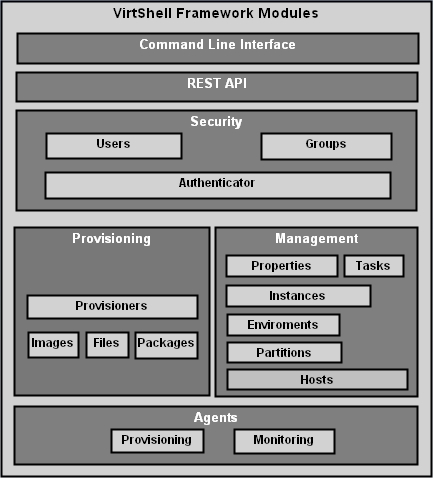
\includegraphics[width = 0.8\textwidth]{../architecture/v1/diagrams/framework}
\end{figure}

Las siguientes secciones detallan los módulos disponibles para cada característica. 

\subsection{Security}
Seguridad consiste de los módulos de \emph{users} (usuarios), \emph{groups} (grupos) y el modulo \emph{authenticator} (de autenticación). El control de los usuarios y grupos son elementos clave en la administración del framework. Los \textbf{Usuarios} pueden ser personas reales, es decir, cuentas ligadas a un usuario físico en particular o cuentas que existen para ser usadas por aplicaciones específicas. \\
\\
Los \textbf{Grupos} son expresiones lógicas de organización, reuniendo usuarios para un propósito común. Los usuarios dentro de un mismo grupo pueden leer, escribir o ejecutar los recursos que pertenecen a ese grupo.\\
\\
El módulo de \textbf{autenticación} soporta el proceso por el cual cuando un usuario se presenta a la aplicación puede validar su identidad. Este módulo es quien decide0 si el usuario tiene permiso para ingresar al sistema y el nivel de acceso a un recurso dado. En el capitulo 4 se detalla el proceso de autenticación y autorización.

\subsection{Managment}
Administración consiste de los modulos \emph{hosts} (anfitriónes), \emph{partitions} (particiones), \emph{enviroments} (ambientes), \emph{instances} (instancias), \emph{properties} (propiedades) y \emph{tasks} (tareas). \\
\\
El módulo de \textbf{anfitriónes} lleva registro de nodos físicos, servidores o máquinas virtuales, que se encuentren conectados a la red y que permitan albergar instancias virtuales. Los anfitriónes son clasificados de acuerdo a diferentes combinaciones de CPU, memoria, almacenamiento y capacidad de trabajo en red, dando flexibilidad para elegir la opcion mas adecuada para las necesidades de las aplicaciones destino. En otras palabras el tipo de anfitrión determina el hardware del nodo físico que sera usado por los recursos virtuales.\\
\\
El módulo de \textbf{particiones} permite dividir los anfitriones en secciones aisladas de disponibilidad. Cada partición puede ser usada para definir áreas geográficas separadas o simplemente para dividir los nodos físicos en subgrupos destinados a diferentes usos o equipos de trabajo o tipos de clientes.\\
\\
El módulo de \textbf{ambientes} permite dividir lógicamente una partición en subredes de trabajo más pequeñas, con lo que se crean grupos más pequeños con diferentes fines. En los ambientes de trabajo se configuran los usuarios que tienen permiso para interactuar trabajar con el.\\
\\
El módulo de \textbf{instancias} es un recurso virtual o máquina virtual o contenedor con parámetros y capacidades definidas en la cual se puede instalar el software deseado. Un usuario puede crear, aprovisionar, actualizar y finalizar instancias en VirtShell tanto como necesite dando la sensación de elasticidad \footnote{La elasticidad es una de las propiedades fundamentales de la nube. La elasticidad consiste en la potencia de escalar los recursos informáticos ampliándolos y reduciéndolos dinámicamente.} de la red.\\
\\
El módulo de \textbf{propiedades} permite consultar información de sistema, de las instancias o de los anfitriones físicos. La información que puede ser consultada es toda aquella que el sistema tenga disponible o que se pueda consultar por medio de comandos de sistema o comandos propios de VirtShell. Ejemplos de información que se puede consultar por medio de las propiedades es porcentajes de memoria y cpu usada, numero de procesos en ejecución, etc. Las propiedades pueden ser consultadas en una sola maquina, o simultáneamente en varias maquinas, o a un conjunto de maquinas de acuerdo a prefijos en su nombre.\\
\\
Finalmente, el módulo de \textbf{tareas} da la información y estado sobre las diferentes tareas o trabajos ejecutados en el sistema. Debido a que el medio para interactuar con los módulos de VirtShell es a través de un API REST, una petición de creación de un nuevo recurso virtual, puede ser largo si el aprovisionamiento involucra varias maquinas. Para evitar, tener una petición esperando respuesta, VirtShell crea una tarea que sera ejecutada de manera asincrónica, dando como respuesta, un identificador de la tarea, para que esta pueda ser consultada posteriormente y conocer el estado de la petición.


\subsection{Provisioning}
Aprovisionamiento consiste de los módulos \emph{provisioners} (aprovisonadores), \emph{images} (imágenes), \emph{files} (archivos) y \emph{packages} (paquetes).\\
\\
El módulo de \textbf{aprovisionadores} define un marco de aprovisionamiento de un recurso virtual y contiene las configuraciones necesarias para apoyar ese marco. La configuración fundamental de un aprovisionador, es la ruta del repositorio git \footnote{git es un software de control de versiones diseñado por Linus Torvalds}, donde se encuentran los scripts y archivos necesarios para realizar el aprovisionamiento. Del mismo modo la forma de ejecutar los scripts, hace parte de la configuración básica. Para ser mas ligero a VirtShell, los scripts de aprovisionamiento, deben estar registrados en un repositorio git público. VirtShell se encarga de descargar el repositorio y de ejecutar los scripts de aprovisionamiento, de acuerdo a la configuración especificada. \\
\\
Adicionalmente, los aprovisonadores cuentan con una manera de especificar las dependencias del nuevo recurso virtual. VirtShell se encarga de resolver las dependencias antes de realizar el aprovisionamiento del nuevo recurso, a su vez, suministra información de ellas a los scripts de aprovisionamiento si estos lo requieren. \\
\\
VirtShell utiliza como lenguaje de referencia, para la creación de scripts de aprovisionamiento, el lenguaje shell. Este cuenta con los recursos suficientes para interactuar con los diferentes sistemas operativos de las instancias. Sin embargo estos comandos se pueden extender usando el paquete de comandos propios de VirtShell, los cuales pueden abstraer muchas de las operaciones del shell. Esto facilita la escritura de los mismos o permite hacerlos independientes del sistema operativo en el cual van a ejecutarse.\\
\\
El módulo de \textbf{imágenes} proporciona la información necesaria de las imágenes que se encuentran registradas en el sistema. Cada vez que se crea un nuevo recurso virtual en un anfitrión, se especifica el nombre de la imagen almacenada en el sistema que sera usada, de una de las que se encuentra en el sistema. \\
\\
Las imágenes que se manejan en VirtShell son de dos tipos: ISO \footnote{Una imagen ISO es un archivo informático donde se almacena una copia o imagen exacta de un sistema de archivos o ficheros de un disco óptico, normalmente un disco compacto (CD) o un disco versátil digital (DVD).} y para contenedores. Las de tipo ISO, se encuentran guardadas en el repositorio de VirtShell, y su uso se enfoca a maquinas virtuales que interactuan con hypervisors. Las imágenes de tipo contenedor, se emplean para tecnologías de visualización de sistema operativo como LXC \footnote{LXC (Linux Containers) es una tecnología de virtualización a nivel de sistema operativo (SO) para Linux. } \cite{lxc16} y Docker \footnote{Docker es un proyecto de código abierto que automatiza el despliegue de aplicaciones dentro de contenedores de software, proporcionando una capa adicional de abstracción y automatización de Virtualización a nivel de sistema operativo en Linux.} \cite{docker16}. Estas son descargadas automáticamente de los repositorios de dominio público de los diferentes proveedores. \\
\\
El módulo de imágenes cuenta también, con la característica de crear automáticamente nuevas imágenes de tipo ISO a partir de las \emph{releases} (liberaciones) base de las diferentes distribuciones de sistemas operativos linux. Una vez creada la nueva ISO esta sera guardada en el repositorio interno para su posterior uso.\\
\\
El módulo de \textbf{archivos} proporciona una manera de almacenar archivos en VirtShell, los cuales pueden ser usados para almacenar 

El módulo de \textbf{archivos} proporciona una manera de almacenar archivos en VirtShell, los cuales pueden ser usados para almacenar información necesaria para crear imágenes o para enviarlos a uno o mas recursos virtuales de manera simultánea en un directorio especificado. Adicionalmente, permite especificar los permisos que tendrán los archivos.\\
\\
El módulo de \textbf{paquetes} facilita realizar funciones tales como la instalación de nuevos paquetes de software y actualización de paquetes existentes en uno o mas recursos virtuales de manera simultanea.


\subsection{Agents}
Los Agentes son servicios que se ejecutan localmente en cada anfitrión, y que se encuentra bajo la gestión de VirtShell. Estos son instalados y configurados en cada anfitrión de manera automática. Los agentes actúan con un cierto grado de autonomía con el fin de completar tareas en nombre del servidor.\\

\chapter{Seguridad}
\label{capseguridad}

\section{Autenticaci'on}
La autenticaci'on es el proceso de demostrar la identidad al sistema. La identidad es un factor importante en las decisiones de control de acceso. Las solicitudes se conceden o deniegan en parte sobre la base de la identidad del solicitante.\\
\\
El VirtShell, el API REST utiliza un esquema HTTP personalizado basado en una llave-HMAC (Hash Message Authentication Code) para la autenticaci'on. Para autenticar una solicitud, primero se concatenan los elementos seleccionados de la solicitud para formar una cadena. A continuaci'on, utiliza una clave secreta de acceso para calcular el HMAC de esa cadena. Informalmente, se le denomina a este proceso \"la firma de la solicitud\", y se denomina a la salida del algoritmo HMAC la "firma", ya que simula las propiedades de seguridad de una firma real. Por 'ultimo, se agrega esta firma como un par'ametro de la petici'on, con la sintaxis descrita en esta secci'on.\\
\\
Cuando el sistema recibe una solicitud fehaciente, se obtiene la clave secreta de acceso que dicen tener, y lo utiliza de la misma manera que se calcula una "firma" del mensaje que recibi'o. A continuaci'on, compara la firma que se calcula con la firma presentada por el solicitante. Si las dos firmas coinciden, el sistema llega a la conclusi'on de que el solicitante debe tener acceso a la clave secreta de acceso, y por lo tanto act'ua con la autoridad del principal al que se emiti'o la clave. Si las dos firmas no coinciden, la solicitud se descarta y el sistema responde con un mensaje de error.\\
\\
Ejemplo de una petici'on autenticada:

\medskip
\begin{lstlisting}
  GET /api/virtshell/packages/{packageId} HTTP/1.1
  Host: host1.edu.co
  Date: Fri, 01 Jul 2011 19:37:58 +0000

  Authorization: 0PN5J17HBGZHT7JJ3X82:frJIUN8DYpKDtOLCwo//yllqDzg= 
\end{lstlisting}

\subsection{Authentication Header}

El API REST utiliza el encabezado de autorizaci'on HTTP para pasar informaci'on de autenticaci'on. Bajo el esquema de autenticaci'on de VirtShell, el encabezado de autorizaci'on tiene la siguiente forma.

\medskip
\begin{lstlisting}
  Authorization: UserId:Signature
\end{lstlisting}
\medskip

Los usuarios tendr'an un ID de clave de acceso (VirtShell Access Key ID) y una clave secreta de acceso (VirtShell Secret Access Key) cuando se registran. Para la petici'on de autenticaci'on, el elemento de VirtShell Access Key Id identifica la clave secreta que se utiliz'o para calcular la firma, y (indirectamente) el usuario que realiza la solicitud.\\
\\
Para la firma de los elementos de la petici'on se usa el RFC 2104 HMAC-SHA1 \cite{rfc2104}, por lo que la parte de la firma de la cabecera autorizaci'on variar'a de una petici'on a otra. Si la solicitud de la firma calculada por el sistema coincide con la firma incluida en la solicitud, el solicitante habr'a demostrado la posesi'on de la clave secreta de acceso. La solicitud ser'a procesada bajo la identidad, y con la autoridad, de la promotora que se emiti'o la clave.\\
\\
A continuaci'on se muestra la pseudo-gram'atica que ilustra la construcci'on de la cabecera de la solicitud de autorizaci'on (
\textbackslash{}n significa el punto de c'odigo Unicode U +000 A com'unmente llamado salto de l'inea).

\medskip
\begin{lstlisting}[basicstyle=\tiny]
  Authorization = VirtShellUserId + ":" + Signature;

  Signature = Base64( HMAC-SHA1( UTF-8-Encoding-Of( YourSecretAccessKeyID, StringToSign ) ) );

  StringToSign = HTTP-Verb + "\n" +
  Host + "\n" +
  Content-MD5 + "\n" +
  Content-Type + "\n" +
  Date + "\n" +
  CanonicalizedResource;

  CanonicalizedResource = <HTTP-Request-URI, from the protocol name up to the query string (resource path)>
\end{lstlisting}

HMAC-SHA1 es un algoritmo definido por la RFC 2104 (ver la RFC 2104 con llave Hashing para la autenticaci'on de mensajes \cite{rfc2104}).\\
\\
El algoritmo toma como entrada dos cadenas de bytes: una clave y un mensaje. Para la solicitud de autenticaci'on, se utiliza la clave secreta (YourSecretAccessKeyID) como la clave, y la codificaci'on UTF-8 del StringToSign como el mensaje. La salida de HMAC-SHA1 es tambi'en una cadena de bytes, llamado el resumen. El par'ametro de la petici'on de la Firma se construye codificada en Base64.

\subsection{Solicitud can'onica para firmar}

Cuando el sistema recibe una solicitud autenticada, compara la solicitud de firma calculada con la firma proporcionada en la solicitud de StringToSign. Por esta raz'on, se debe calcular la firma con el mismo m'etodo utilizado por VirtShell. A este proceso de poner una solicitud en una forma acordada para la firma se denomino "canonizaci'on".

\subsection{Tiempo de sello}

Un sello de tiempo v'alido (utilizando el HTTP header Date) es obligatorio para solicitudes autenticadas. Por otra parte, el tiempo del sello enviado por un usuario que se encuentra incluido en una solicitud autenticada debe estar dentro de los 15 minutos de la hora del sistema cuando se recibe la solicitud. En caso contrario, la solicitud fallar'a con el c'odigo de estado de error RequestTimeTooSkewed. La intenci'on de estas restricciones es limitar la posibilidad de que solicitudes interceptadas pueden ser reproducidos por un adversario.Para una mayor protecci'on contra las escuchas, se debe utilizar el transporte HTTPS para solicitudes autenticadas.

\subsection{Ejemplos de autenticaci'on}

\scriptsize
\captionof{table}{Ejemplos de autenticaci'on}
\begin{tabular}{|l|l|} \hline
\textbf{Parametro} & \textbf{Valor} \\ \hline
VirtShellUserId  & 13010f3e-3f46-4889-b989-592ce8fb30c6 \\ \hline
\multicolumn{1}{|m{3.5cm}|}{VirtShellSecretAccessKey} & 
\multicolumn{1}{m{9cm}|} {
                            \raggedright c991f519-bed0-4dab-9165-6d3f722dc845 \\
                            \textbf{Base64:} \\ Yzk5MWY1MTktYmVkMC00ZGFiLTkxNjUtNmQ5ZjcyMmRjODQ1
                          } \tabularnewline \hline
\end{tabular}
\normalsize

\subsubsection{Ejemplo de un objeto con GET}

Este es un ejemplo que consulta por un host dado su identificador. \\
\\
\vspace{1cm}
\scriptsize
\captionof{table}{Autenticaci'on de un objeto con el método GET}
\begin{tabular}{|l|l|} \hline
\textbf{Request} & \textbf{StringToSign} \\ \hline
\multicolumn{1}{|m{7.5cm}|}{
      \raggedright GET /api/virtshell/hosts/5713b48a-8d73-11e5-8994-feff819cdc9f HTTP/1.1 \\
      Host: host1.edu.co \\
      Date: Tue, 27 Mar 2007 19:36:42 +0000 \\
      Authorization: 13010f3e-3f46-4889-b989-592ce8fb30c6: \\
      Yzk5MWY1MmVkMC00ZGFiLTtNmQ5ZjcyMmRjODQ1 } & 
\multicolumn{1}{m{8cm}|}{
      \raggedright GET\textbackslash{}n \\
      host1.edu.co\textbackslash{}n \\
      \textbackslash{}n \\
      \textbackslash{}n \\
      Tue, 27 Mar 2007 19:36:42 +0000\textbackslash{}n \\ 
      /api/virtshell/hosts/5713b48a-8d73-11e5-8994-feff819cdc9f} \tabularnewline \hline
\end{tabular}
\normalsize

\subsubsection{Ejemplo de un objeto con DELETE}

Este ejemplo remueve un usuario.\\
\\
\vspace{1cm}
\scriptsize
\captionof{table}{Autenticaci'on de un objeto con el método DELETE}
\begin{tabular}{|l|l|} \hline
\textbf{Request} & \textbf{StringToSign} \\ \hline
\multicolumn{1}{|m{7.4cm}|}%
{\raggedright DELETE /api/virtshell/users/5fd13cc8-8d73-11e5-8994-feff819cdc9f HTTP/1.1 \\
 Host: host1.edu.co \\
 Date: Tue, 27 Mar 2007 21:20:27 +0000 \\
 Authorization: 13010f3e-3f46-4889-b989-592ce8fb30c6: Yzk5MWY1MmVkMC00ZGFiLTtNmQ5ZjcyMmRjODQ1 } & \multicolumn{1}{m{8cm}|}%
{\raggedright DELETE\textbackslash{}n \\
 host1.edu.co\textbackslash{}n \\
 \textbackslash{}n \\
 \textbackslash{}n \\
 Tue, 27 Mar 2007 21:20:27 +0000\textbackslash{}n \\ /api/virtshell/users/5fd13cc8-8d73-11e5-8994-feff819cdc9f} \tabularnewline \hline
\end{tabular}

\normalsize
\section{Autorización}
VirtShell es un framework multi-usuario que ofrece protecci'on a recursos basado en los conceptos de permisos de Unix. El mecanismo de protección determina que usuarios están autorizados para acceder a los recursos de: archivos, imágenes, instancias y aprovisionadores, presentes en el sistema. \\
\\
Al igual que en Unix, la técnica usada para ofrecer protección a los recursos consiste en hacer que el acceso dependa de la identidad del usuario. El esquema usado es una lista de acceso condensada por cada recurso que se desea proteger. La lista de acceso se divide en tres grupos de caracteres, representando los permisos del usuario propietario, del grupo propietario, y de los otros, respectivamente, como se muestra en la tabla \ref{tab:permisos}.

\begin{center}
 \captionof{table}{Tipos de permisos}
 \label{tab:permisos}
 \begin{tabular}{| c | p{2.2cm} |}
 \hline
  \rowcolor{blueapi}
  \textbf{Permisos} & \textbf{Pertenece}  \\ [0.2ex] 
  \hline\hline
  rwx------ &  usuario \\
  \hline
  ---r-x--- & grupo \\  
  \hline
  ------r-x & otros \\
  \hline
\end{tabular}
\end{center}

Por ejemplo, los caracteres -rw-r--r-- indican que el usuario propietario del recurso tiene permisos de lectura y escritura, pero no de ejecución (rw-), mientras que los usuarios que pertenecen al grupo propietario y los demás usuarios solo tienen permiso de lectura (r-- y r--). Mientras tanto, los caracteres rwxrwx--- indican que el usuario propietario del recurso y todos los usuarios que pertenecen al grupo propietario tienen permisos de lectura, escritura y ejecución (rwx y rwx), mientras que los demás usuarios no pueden acceder (---). \\
\\
La siguiente una descripción de los tres atributos básicos que se manejan en VirtShell:

\begin{center}
 \captionof{table}{Atributos básicos}
 \begin{tabular}{| l | p{12cm} |}
 \hline
  \rowcolor{blueapi}
  \textbf{Atributo} & \textbf{Descripción}  \\ [0.2ex] 
  \hline\hline
  Lectura &  Permite a un usuario ver el contenido de cualquier recurso. \\
  \hline
  Escritura & Permite a un usuario crear, modificar y eliminar un recurso. \\  
  \hline
  Ejecución & Permite a un usuario ejecutar instancias virtuales. 
  por ejemplo: iniciar, detener, pausar, clonar o actualizar paquetes. 
   (El usuario también debe tener permiso de lectura). \\
  \hline
\end{tabular}
\end{center}

Un ejemplo que muestra la asignación de permisos para una instancia es el siguiente:

\medskip
\begin{lstlisting}[style=json]
curl -sv -X POST \
  -H 'accept: application/json' \
  -H 'X-VirtShell-Authorization: UserId:Signature' \
  -d '{ "name": "transactional_log",
        "memory": 1024,
        "cpus": 2,
        "hdsize": "2GB",
        "operating_system": "ubuntu_server_14.04.2_amd64",
        "description": "Server transactional only for store logs", 
        "provisioner": "all_backend",
        "host_type": "GeneralPurpose",
        "driver": "lxc",
        "permissions": "rwx------"
      }' \
   'http://localhost:8080/virtshell/api/v1/instances'
\end{lstlisting}

Como se observa, en la información enviada en la petición POST al servidor HTTP de VirtShell, el usuario esta solicitando crear una instancia en donde especifica en los tres primeros caracteres que solo el como propietario tiene permiso para interactuar con ella. Cabe aclarar que si no se especifican los permisos en la información enviada, VirtShell asigna todos los permisos al recurso creado dejándolo publico para todos los usuarios del sistema.

\chapter{Adminsitración}
\label{capadministracion}

La capa de Administración de VirtShell proporciona una infraestructura de servicios para la gestión de cualquier dispositivo registrado y creado a traves del sistema. Este capítulo busca darle explicación a las funcionalidades de administración para utilizarlas en su beneficio.

\section{Particiones, anfitriones y Ambientes en VirtShell}
En VirtShell hay tres conceptos que son muy importantes y se extiende a través de todos los servicios, y que simplemente no puede dejar de tener en cuenta: Las particiones, los ambientes y las instancias. Las tres se asocian con la mayoría de las cosas en VirtShell, y el dominio de ellos es crucial para una buena administración de los dispositivos. 

\subsection{Particiones}
Las particiones consisten de uno o más anfitriones, los cuales pueden ser nodos físicos, servidores o incluso máquinas virtuales. El objetivo principal que busca una partición, es organizar las máquinas que albergaran recursos virtuales en partes aisladas de las demás. Estas partes pueden pueden estar ubicadas en un mismo sitio físico o por el contrario puede estar distribuidas es diferentes zonas geográficas de todo el mundo.\\
\\
Si solo se cuenta con un numero fijo de maquinas (o anfitriones) ubicadas en un mismo sitio físico como por ejemplo un datacenter \footnote{Un data center también llamado centro de datos es un espacio acondicionado especialmente para contener a todos los equipos y sistemas de TI}, lo que se obtiene con las particiones es la posibilidad de dividir esas maquinas en subgrupos que puedan ser destinados para diferentes equipos o divisiones dentro de una organización.\\ 
\\
Al contar con maquinas distribuidas en diferentes zonas geográficas la elección de una partición u otra se basa principalmente en la cercanía de los visitantes o clientes, ya que a menor distancia entre los servidores y ellos, menores son los tiempos de respuesta y mejor la experiencia de usuario.\\
\\
Las particiones también favorecen la disponibilidad. Si distribuye sus instancias a través de múltiples particiones y una instancia falla, puede diseñar su aplicación para que una instancia en otra partición pueda atender las peticiones.\\
\\
Cuando se crea una nueva partición, VirtShell la crea completamente vaciá, sin anfitriones. Para asociar anfitriones a una partición se debe crear un anfitrión y vincularlo con la partición como se vera mas adelante en este mismo capítulo. Un ejemplo de como crear una partición usando el API se muestra en el siguiente código:

\begin{lstlisting}[style=json, caption=Petición HTTP para crear una partición]
curl -sv -X POST \
  -H 'accept: application/json' \
  -H 'X-VirtShell-Authorization: UserId:Signature' \
  -d '{
       "name": "development_co",
       "description": "Collection of servers oriented to development team in colombia."
      }' \
   'http://localhost:8080/api/virtshell/v1/partitions'
\end{lstlisting}


\subsection{Asociación de anfitriones a particiones}
Los anfitriones no son mas que nodos físicos, servidores o máquinas virtuales, que alojaran recursos virtuales. VirtShell ofrece la posibilidad de clasificarlos de acuerdo a combinaciones de capacidad de CPU, memoria, almacenamiento y red. El objetivo que busca la clasificación es proporcionar flexibilidad para elegir la combinación de recursos adecuada para las aplicaciones.\\
\\
Los tipos de anfitriones se agrupan en familias basadas en perfiles de aplicación de destino. Estos grupos incluyen: de propósito general, con procesadores de alto desempeño, de memoria optimizada, de almacenamiento optimizado.

\begin{description}
\item [Propósito general] Esta familia proporciona un equilibrio de recursos informáticos, de memoria y red, por lo que constituye una buena opción para muchas aplicaciones.
\item [Procesadores de alto desempeño] Esta familia ofrece procesadores que alcanzan alto desempeño en tareas complejas.
\item [Memoria optimizada] Esta familia esta optimizada para aplicaciones con un uso intenso de la memoria.
\item [Almacenamiento optimizado] Esta familia promete anfitriones con alta capacidad de almacenamiento, optimizado para un desempeño de E/S muy alto.
\end{description}

Cuando se crea un anfitrión en VirtShell este debe ser asociado a una sola partición, asignándole un tipo, con alguno de los mencionados anteriormente, estableciendo las capacidad de disco y memoria RAM con las que cuenta,  
indicando también el sistema operativo y las ip con las que se conecta a la red. Una vez el anfitrión es creado en el sistema este queda asignado a la partición elegida. El siguiente ejemplo muestra como crear un anfitrión usando el API:

\begin{lstlisting}[style=json, caption=Petición HTTP para crear un host]
curl -sv -X POST \
  -H 'accept: application/json' \
    -H 'X-VirtShell-Authorization: UserId:Signature' \
  -d '{"name": "host-01-pdn",
       "os": "Ubuntu_12.04_3.5.0-23.x86_64",
       "memory": "16GB",
       "capacity": "120GB",
       "enabled": "true",
       "type" : "GeneralPurpose",
       "local_ipv4": "15.54.88.19",
       "local_ipv6": "ff06:0:0:0:0:0:0:c3",
       "public_ipv4": "10.54.88.19",
       "public_ipv6": "yt06:0:0:0:0:0:0:c3",
       "partition": "development_co"}' \
   'http://localhost:8080/virtshell/api/v1/hosts'
\end{lstlisting}

\vspace{5mm}

En este ejemplo se muestra la creación de un anfitrión con nombre host-01-pdn que esta clasificado como de uso general y que queda asociado a la partición development\_co creada en la sección anterior.\\
\\
Al consultar la partición nuevamente por medio del API se puede observar como el anfitrión se encuentra asociado a la partición developtment\_co. En la siguiente consulta al API se muestra el resultado de la asociación:

\vspace{5mm} 

\begin{lstlisting}[style=json, , caption=Petición HTTP para consultar una partición por su nombre]
curl -sv -H 'accept: application/json' 
     -H 'X-VirtShell-Authorization: UserId:Signature' \ 
     'http://<host>:<port>/api/virtshell/v1/partitions/development_co'
\end{lstlisting}

\vspace{5mm}

Respuesta:

\vspace{5mm}

\begin{lstlisting}[style=json]
HTTP/1.1 200 OK
Content-Type: application/json
{
  "uuid": "efa1777c-cad7-11e5-9956-625662870761",
  "name": "development_co",
  "description": "Collection of servers oriented to development team in colombia.", 
  "hosts": [ "host-01-pdn" ],  
  "created": {"at":"1429207233", 
              "by":"1a900cdc-cad8-11e5-9956-625662870761"}
}
\end{lstlisting}

\vspace{5mm}

Adicionalmente, cuando un anfitrión es agregado a una partición, VirtShell instala automáticamente los agentes  que realizaran tareas de aprovisionamiento y monitoreo. Los agentes se explicaran mas adelante.

\subsection{División de particiones en ambientes}
Las particiones se refieren a la forma de organizar lugares físicos. Los ambientes por el contrario, son lugares lógicos y aislados dentro de una partición. Cada partición puede estar compuesta por uno o varios ambientes, y un ambiente puede contener uno o mas instancias. Cada ambiente pertenece a una sola partición. La figura \ref{fig:enviroment} muestra un ejemplo de como dos particiones contiene varios ambientes destinados a equipos de trabajo diferentes. \\

\begin{figure}[h]
    \centering
  \caption{Ejemplo de ambientes en un partición}
  \label{fig:enviroment}
  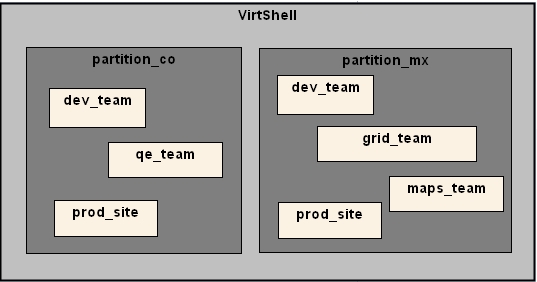
\includegraphics[width = 0.95\textwidth]{../architecture/v1/diagrams/enviroments}
\end{figure}

Un ejemplo de como crear un ambiente asociado a una partición usando el API se muestra en el siguiente código:

\begin{lstlisting}[style=json, caption=Petición HTTP para crear un ambiente]
curl -sv -X POST \
  -H 'accept: application/json' \
  -H 'X-VirtShell-Authorization: UserId:Signature' \
  -d '{
       "name": "bigdata_laboratory",
       "description": "Collection of servers oriented to big data.", 
       "partition": "bogota_partition_co"
      }' \
   'http://localhost:8080/api/virtshell/v1/enviroments'
\end{lstlisting}

\section{Instancias}
A un servidor virtual en VirtShell, se le denomina instancia, las cuales pueden ser maquinas virtuales que corren sobre algún hipervisor o también pueden ser contenedores que se ejecutan directamente sobre el sistema operativo del anfitrión. \\
\\
La elección de la tecnología de virtualización depende de las preferencias u objetivos que se busque con las aplicaciones de la instancia. En la actualidad VirtShell soporta Virtualbox como hipervisor para maquinas virtuales y para los contenedores soporta LXC \footnote{LXC (Linux Containers) es una tecnología de virtualización en el nivel de sistema operativo (SO) para Linux. } \cite{lxc16} y Docker \footnote{Docker es un proyecto de código abierto que automatiza el despliegue de aplicaciones dentro de contenedores de software, proporcionando una capa adicional de abstracción y automatización de Virtualización a nivel de sistema operativo en Linux.} \cite{docker16}.\\
\\
Las instancias son designadas a solo ambiente de trabajo en el momento de ser creadas. En el instante de su creación, se debe especificar las características de CPU, memoria y capacidad de disco que se desea. De igual manera, se configura el sistema operativo, los permisos para los demás usuarios del sistema, el tipo de anfitrión que necesita y la tecnología que se desea usar para virtualizar.

\subsection{Creación de instancias en un ambiente}
Cuando se recibe una solicitud de creación de una instancia, VirtShell selecciona un anfitrión, de los que se encuentran configurados en la partición a la cual pertenece el ambiente donde se quiere crear la instancia. En la solicitud de creación se debe especificar el tipo de anfitrión que se requiere para el correcto funcionamiento de las aplicaciones que se ejecutaran ahí. Si la partición no cuenta con el tipo de anfitrión solicitado, se rechazara la petición detallando el inconveniente. Si por el contrario la selección del anfitrión es exitosa, VirtShell procede a enviar la solicitud al agente de aprovisionamiento del anfitrión escogido. \\
\\
Debido a que una solicitud de aprovisionamiento puede involucrar mas de una instancia, el servidor de VirtShell responde la solicitud de aprovisionamiento con el estado de \emph{in-progress} (en progreso) y a su vez con el identificador de una tarea. La tarea será ejecutada de manera asincrónica y el usuario por medio del API REST puede consultar el estado y avance de la misma (Las tareas se ampliaran en la siguiente sección).\\
\\
Un ejemplo de la creación de una instancia usando el API se muestra en el siguiente código:

\begin{lstlisting}[style=json, caption=Petición HTTP para crear una instancia]
curl -sv -X POST \
  -H 'accept: application/json' \
  -H 'X-VirtShell-Authorization: UserId:Signature' \
  -d '{ "name": "transactional_log",
        "memory": 8024,
        "cpus": 2,
        "hdsize": "20GB",
        "enviroment": "development_co",
        "operating_system": "ubuntu_server_14.04.2_amd64",
        "description": "Server transactional only for store logs", 
        "provisioner": "all_backend",
        "host_type": "GeneralPurpose",
        "driver": "lxc"
      }' \
   'http://localhost:8080/api/virtshell/v1/instances'
\end{lstlisting}

\vspace{5mm}

En esta solicitud HTTP se observa que la instancia a crear debe tener el  sistema operativo es Linux Ubuntu, contar con 8 Gigabytes de memoria RAM, dos núcleos, 20 Gigabyte de disco duro, y que debe ser creada en el ambiente de nombre development\_co en una maquina física de uso general. Adicionalmente la instancia debe ser un contenedor que se ejecute sobre LXC.\\
\\
Si la solicitud de las características es exitosa, el servidor responderá de la siguiente manera:

\vspace{5mm}

\begin{lstlisting}[style=json, caption=Ejemplo de respuesta HTTP a la solicitud de crear una instancia]
HTTP/1.1 200 OK
Content-Type: application/json
{ "create": "in progress", "task": "bbf6669b-1b83-4fe7-ae2a-2b31738c4165" }
\end{lstlisting}

Si por el contrario, la solicitud no es exitosa, el servidor responderá con el respectivo código de error HTTP y la razón por la cual no se pudo procesar exitosamente la petición. Un ejemplo de una petición no procesada es la siguiente: 

\vspace{5mm}

\begin{lstlisting}[style=json, caption=Ejemplo de respuesta HTTP con error a la solicitud de crear una instancia]
HTTP/1.1 500 OK
Content-Type: application/json
{ "create": "error", "reason": "The enviroment doesn't have the host_type requested" }
\end{lstlisting}

\vspace{5mm}

Adicional a la creación de instancias, el API REST de VirtShell proporciona URIs para su gestión. Las operaciones sobre el ciclo de vida de una instancia que permite realizar son: iniciar, detener, reiniciar, cerrar y clonar. Así mismo, el API posibilita la fácil y rápida búsqueda de una o mas instancias.  

\section{Tareas}
Una tarea es una actividad asincrónica, que se ejecuta en \emph{background} (segundo plano), y se crea de manera automática cuando se solicita una acción al servidor, y esta pueda tomar un largo periodo de tiempo para completar su trabajo.\\
\\
Las tareas asíncronas resuelven los problemas relacionados con los tiempos de espera de las conexiones, los tiempos de espera de la solicitudes o los tiempos de vida de las peticiones HTTP antes de que estas sean cerradas por el servidor de aplicaciones web o por el navegador de manera automática de acuerdo a sus parámetros de configuración.\\
\\
Las operaciones de larga duración en VirtShell son las que involucran acciones en las instancias. Debido a que estas ultimas pueden estar físicamente lejanas del servidor, el tiempo de espera de una petición HTTP puede incrementarse lo suficiente para que esta sea finalizada por el servidor web. Asimismo, las operaciones de aprovisionamiento de las instancias, las cuales consisten principalmente en instalación y configuración de paquetes son tareas que involucran componentes realizados por terceros sobre los cuales no se tiene control sobre sus tiempos de respuesta.\\
\\
Cuando VirtShell recibe una petición y esta es considerada de larga duración, en el cuerpo de la respuesta se enviá la acción recibida con el estado de \emph{in progress} acompañado del identificador único UUID \footnote{UUID son las siglas en inglés del Identificador Universalmente Único.} de la tarea. Por ejemplo, si se recibe una petición de instalación de un paquete en una o mas instancias, la respuesta HTTP seria de la siguiente forma:

\begin{lstlisting}[style=json, caption=Ejemplo de respuesta HTTP referenciando a una tarea]
HTTP/1.1 200 OK
Content-Type: application/json
{ "install-package": "in progress", "task": "908b4d78-8b7a-40d7-9ecf-5036eeb5526b" }
\end{lstlisting}

\vspace{5mm}

Para consultar por el estado de una tarea, se invoca el API de VirtShell, enviando en la url, el identificador UUID recibido de la primera petición, el servidor responderá con un documento en formato JSON detallando la tarea y su estado. El siguiente es un ejemplo de una consulta sobre una tarea y la respuesta del servidor:

\vspace{5mm}

\begin{lstlisting}[style=json, caption=Ejemplo de consulta de una tarea]
curl -sv -H 'accept: application/json' 
     -H 'X-VirtShell-Authorization: UserId:Signature' \ 
     'http://<host>:<port>/api/virtshell/v1/tasks/908b4d78-8b7a-40d7-9ecf-5036eeb5526b'
\end{lstlisting}

\vspace{5mm}

Respuesta:

\vspace{5mm}


\begin{lstlisting}[style=json, caption=Ejemplo del detalle de una tarea]
HTTP/1.1 200 OK
Content-Type: application/json
```
```json
{
  "uuid": "908b4d78-8b7a-40d7-9ecf-5036eeb5526b",
  "description": "install-package in instance database_01",
  "status" : "installing",
  "created": {"at":"1429207233", "by":"92d30f0c-8c9c-11e5-8994-feff819cdc9f"},
  "last_update": "1429207435",
  "log": "installing package couchdb"
}
\end{lstlisting}


\section{Propiedades}

\chapter{Aprovisionamiento}
\label{capaprovisionamiento}

VirtShell cuenta con una colección de recursos, que permite el aprovisionamiento de instancias,independientemente de la infraestructura de visualización que se use para estas. El conjunto de recursos de esta capa, esta diseñado para que sea una solución sencilla de usar, fiable y repetible, con una curva de aprendizaje muy baja para los administradores, desarrolladores y administradores de TI. Este capítulo busca describir todo lo que se requiere para llevar a cabo un correcto aprovisionamiento en las instancias creadas a traves el sistema.

\section{Imágenes}


\section{Aprovisionadores}

\section{Instalación de paquetes y archivos}




\chapter{Agentes}
\label{capagents}

En este capítulo se definen los elementos que apoyan a VirtShell a realizar su trabajo en cada uno de los anfitriones. Estos elementos son llamados agentes.\\
\\
Los agentes son servicios que se ejecutan localmente en cada anfitrión. VirtShell instala y configura los agentes en cada uno de los anfitriones de manera automática, liberando de esta tarea al administrador del sistema. Existen tres tipos de agentes: de aprovisionamiento, monitoreo y administración.

\begin{description}
\item [Agente de Aprovisionamiento]
El agente de aprovisionamiento se encarga de instalar y configurar: paquetes, librerías y aplicaciones en las instancias. 
\item [Agente de Monitoreo]
El agente de monitoreo es completamente autónomo y sus funciones consisten en supervisar al agente de aprovisionamiento y reportar el estado de salud de los anfitriones e instancias que se encuentran creados en su interior. 
\item [Agente de Administración]
El agente de administración se encarga de gestionar las instancias, permitiendo detener, iniciar, clonar, eliminar y obtener información especifica de cada instancia que se ejecuta en el anfitrión.
\end{description}
\chapter{API}
\label{capapi}

En este capítulo se detalla el API REST de VirtShell, en el se describen cada uno de los métodos HTTP que soportan los módulos, sus recursos en formato JSON y adicionalmente se ofrecen ejemplos detallados de cada una de las peticiones HTTP.\\

\section{Definición de API}
API significa ``Application Programming Interface", y como término, especifica cómo debe interactuar el software.\\
\\
En términos generales, cuando nos referimos a las API de hoy, nos referimos más concretamente a las API web, que son manejadas a través del protocolo de transferencia de hipertexto (HTTP). Para este caso específico, entonces, una API especifica cómo un consumidor puede consumir el servicio que el API expone: cuales URI están disponibles, qué métodos HTTP puede utilizarse con cada URI, que parámetros de consulta se acepta, lo que los datos que pueden ser enviados en el cuerpo de la petición, y lo que el consumidor puede esperar como respuesta.

\subsection{VirtShell API REST}
En el VirtShell API REST un usuario enviá una solicitud al servidor para realizar una acción determinada (como la creación, recuperación, actualización o eliminación de un recurso virtual), y el servidor realiza la acción y enviá una respuesta, a menudo en la forma de una representación del recurso especificado.\\
\\
En el VirtShell API, el usuario especifica una acción con un verbo HTTP como POST, GET, PUT o DELETE. Especificando un recurso por un URI único global de la siguiente forma: \\
\\
https://[host]:[port]/virtshell/api/v1/resourcePath?parameters\\
\\
Debido a que todos los recursos del API tienen una única URI HTTP accesible, REST permite el almacenamiento en cache de datos y esta optimizado para trabajar con una infraestructura distribuida de la web.\\
\\
En esta sección se detalla los recursos y operaciones que puede realizar un usuario del API para realizar aprovisionamientos automáticos desde cualquier plataforma de desarrollo. El VirtShell API provee acceso a los objetos en el VirtShell Server, esto incluye los hosts, imágenes, archivos, templates, aprovisionadores, instancias, grupos y usuarios. Por medio del API podrá crear ambientes, maquinas virtuales y contenedores personalizados, realizar configuraciones y administrar los recursos físicos y virtuales de manera programática. \\

\section{Formato de entrada y salida}
JSON (JavaScript Object Notation) es un formato de datos común, independiente del lenguaje que proporciona una representación de texto simple de estructuras de datos arbitrarias. Para obtener mas información, ver json.org.\\
\\
El VirtShell API solo soporta el formato json para intercambio de información. Cualquier solicitud que no se encuentre en formato json resultara en un error con código 406 (Content Not Acceptable Error).

\section{Codigos de error}
Aqui se presenta una lista de codigos de error que pueden resultar de una petici'on al API en cualquier recurso.

\begin{itemize}
\item \textbf{400 Bad Request} La solicitud no pudo ser procesada con 'exito porque el URI no era v'alido. El cuerpo de la respuesta contendr'a una raz'on del fracaso de la petici'on. Esta respuesta indica error permanente.

\item \textbf{403 Forbidden} La solicitud no pudo ser procesada con 'exito porque la identidad del usuario no tiene acceso suficiente para procesar la solicitud. Esta respuesta indica error permanente.

\item \textbf{406 Content Not Acceptable} Un recurso genera este error de acuerdo al tipo de cabeceras enviadas en la petici'on. Esta respuesta indica un error permanete e indica un formato de salida no soportado. La respuesta de este tipo de error no contiene un contenido debido a la inhabilidad del servidor para generar una respuesta en el formato solicitado.

\item \textbf{404 Not Found} La solicitud no pudo ser procesada con 'exito porque la solicitud no era v'alida. Lo m'as probable es que no se encontró la url. Esta respuesta indica error permanente.

\item \textbf{500 Server Error} La solicitud no pudo ser procesada debido a que el servidor encontr'o una condici'on inesperada que le impidi'o cumplir con la petici'on.

\item \textbf{501 Not Implemented} La solicitud no se pudo completar porque el servidor o bien no reconoce el m'etodo de petici'on o el recurso solicitado no existe.

\end{itemize}

Los errores que no sean de codigo 406 (Content Not Acceptable) contienen una respuesta en formato json, que contiene un breve mensaje explicado el error con m'as detalle. Por ejemplo, una consulta POST /virtshell/api/v1/hosts, con un cuerpo vacio, dar'ia lugar a la siguiente respuesta:

\vspace{1cm}
\begin{lstlisting}[style=json]
HTTP/1.1 400 Bad Request
Content-Type: application/json

{"error": "Missing input for create instance"}
\end{lstlisting}

\section{API Resources}

\subsection{Groups}
Representan los grupos registrados en VirtShell. Los metodos soportados son:

\begin{center}
 \begin{tabular}{| l | l | l | l |}
 \hline
  \rowcolor{blueapi}
  \textbf{Acci'on} & \textbf{Metodo HTTP} & \textbf{Solicitud HTTP} & \textbf{Descripci'on} \\ [0.5ex] 
  \hline\hline
  get & GET & /users/id & Gets one group by ID. \\
  \hline
  list & GET & /hosts & Retrieves the list of groups. \\  
  \hline
  create & POST & /users/ & creates a new group. \\
  \hline
  delete & DELETE & /users/id & Deletes an existing group. \\
  \hline
\end{tabular}
\end{center}

\vspace{1cm}
Representaci'on del recurso de un grupo:
\vspace{1cm}

\begin{lstlisting}[style=json]
{
  "uuid": "ab8076c0-db91-11e2-82ce-0002a5d5c51b",
  "name": "web_development_team",
  "users": [ ... list of members of the group ...],  
  "created":[ {"at":"timestamp"}, {"by":user_id}]
}
\end{lstlisting}

Ejemplo:

\medskip
\begin{lstlisting}[style=json]
{
  "uuid": "ab8076c0-db91-11e2-82ce-0002a5d5c51b",
  "name": "web_development_team",
  "users": [ 
      {"username": "user1", "id": "a146cae4-8c90-11e5-8994-feff819cdc9f"},
      {"username": "user2", "id": "a146d00c-8c90-11e5-8994-feff819cdc9f"}
  ]
  "created":[{"at":"1447696674"}, {"by":"a379e8e6-8c8b-11e5-8994-feff819cdc9f"}]
}
\end{lstlisting}

\subsubsection{Ejemplos de peticiones HTTP}

\paragraph{Crear un nuevo grupo - POST /virtshell/api/v1/grupos} ~\\

\begin{lstlisting}[style=json]
curl -X POST \
  -H 'accept: application/json' \
  -H 'X-VirtShell-Authorization: UserId:Signature' \
  -H "Content-Type: multipart/form-data" \
  -d '{"name": "database_team"}' \
  'http://<host>:<port>/api/virtshell/v1/groups'
\end{lstlisting}

\vspace{1cm}
Respuesta:
\vspace{1cm}

\begin{lstlisting}[style=json]
HTTP/1.1 200 OK
Content-Type: application/json
{ "create": "success" }
\end{lstlisting}

\paragraph{Obtener un grupo - GET /virtshell/api/v1/groups/:id} ~\\

\begin{lstlisting}[style=json]
curl -sv -H 'accept: application/json' 
     -H 'X-VirtShell-Authorization: UserId:Signature' \ 
     'http://<host>:<port>/api/virtshell/v1/groups/?id=ab8076c0-db91-11e2-82ce-0002a5d5c51b'
\end{lstlisting}

\vspace{1cm}
Respuesta:
\vspace{1cm}

\begin{lstlisting}[style=json]
HTTP/1.1 200 OK
Content-Type: application/json
{
  "uuid": "ab8076c0-db91-11e2-82ce-0002a5d5c51b",
  "name": "web_development_team",
  "users": [ 
      {"username": "user1", "id": "a146cae4-8c90-11e5-8994-feff819cdc9f"},
      {"username": "user2", "id": "a146d00c-8c90-11e5-8994-feff819cdc9f"}
  ]
  "created":[{"at":"1447696674"}, {"by":"a379e8e6-8c8b-11e5-8994-feff819cdc9f"}]
}
\end{lstlisting}

\paragraph{Obtener todos los grupos - GET /virtshell/api/v1/groups} ~\\

\begin{lstlisting}[style=json]
curl -sv -H 'accept: application/json' 
     -H 'X-VirtShell-Authorization: UserId:Signature' \ 
     'http://localhost:8080/api/virtshell/v1/groups'
\end{lstlisting}

\vspace{1cm}
Respuesta:
\vspace{1cm}

\begin{lstlisting}[style=json]
HTTP/1.1 200 OK
Content-Type: application/json
{
  "groups": [
    {
      "uuid": "ab8076c0-db91-11e2-82ce-0002a5d5c51b",
      "name": "web_development_team",
      "users": [ 
          {"username": "user1", "id": "a146cae4-8c90-11e5-8994-feff819cdc9f"},
          {"username": "user2", "id": "a146d00c-8c90-11e5-8994-feff819cdc9f"}
      ],     
      "created":[{"at":"1447696833"}, {"by":"d2372efa-8c8b-11e5-8994-feff819cdc9f"}]
    },
    {
      "uuid": "a379f19c-8c8b-11e5-8994-feff819cdc9f",
      "name": "math_team",
      "users": [ 
          {"username": "user3", "id": "a146cae4-8c90-11e5-8994-feff819cdc9f"}
      ],     
      "created":[{"at":"1421431233"}, {"by":"18489280-8c91-11e5-8994-feff819cdc9f"}]
    },
    {
      "uuid": "a379f3d6-8c8b-11e5-8994-feff819cdc9f",
      "name": "chemical_team",
      "users": [ 
          {"username": "user4", "id": "F8489280-8c91-11e5-8994-feff819cdc9f"},
          {"username": "user5", "id": "18489780-8c91-11e5-8994-feff819cdc9f"}
      ],       
      "created":[{"at":"1424109633"}, {"by":"d2373576-8c8b-11e5-8994-feff819cdc9f"}]
    },        
}  
\end{lstlisting}

\paragraph{Eliminar un grupo - DELETE /virtshell/api/v1/groups/:id} ~\\

Para eliminar un grupo se debe tener en cuenta que no debe tener usuarios asociados a el.

\begin{lstlisting}[style=json]
curl -sv -X DELETE \
   -H 'accept: application/json' \
   -H 'X-VirtShell-Authorization: UserId:Signature' \
   'http://localhost:8080/api/virtshell/v1/groups?id=73cff0b0-8c8e-11e5-8994-feff819cdc9f'
\end{lstlisting}

\vspace{1cm}
Respuesta:
\vspace{1cm}

\begin{lstlisting}[style=json]
HTTP/1.1 200 OK
Content-Type: application/json
```
```json
{ "delete": "success" }
\end{lstlisting}

\subsection{Users}
Representan los usuarios registrados en VirtShell. Los metodos soportados son:

\begin{center}
 \begin{tabular}{| l | l | l | l |}
 \hline
  \rowcolor{blueapi}
  \textbf{Acci'on} & \textbf{Metodo HTTP} & \textbf{Solicitud HTTP} & \textbf{Descripci'on} \\ [0.5ex] 
  \hline\hline
  get & GET & /users/id & Gets one user by ID. \\
  \hline
  create & POST & /users/ & creates a new user. \\
  \hline
  list & GET & /users & Retrieves the list of users. \\  
  \hline
  delete & DELETE & /users/id & Deletes an existing user. \\
  \hline  
  update & PUT & /users/id & Updates an existing user. \\ [1ex]  
  \hline
\end{tabular}
\end{center}

\vspace{1cm}
Representaci'on del recurso de un usuario:
\vspace{1cm}

\begin{lstlisting}[style=json]
{
  "uuid": "ab8076c0-db91-11e2-82ce-0002a5d5c51b",
  "username": "virtshell",
  "type": "system/regular",
  "login": "user@mail.com",
  "groups": [ ... list of users ...],
  "created": {"at": timestamp, "by": user_uuid},
  "modified": {"at": timestamp, "by": user_uuid}
}
\end{lstlisting}

Ejemplo:

\medskip
\begin{lstlisting}[style=json]
{
  "uuid": "ab8076c0-db91-11e2-82ce-0002a5d5c51b",
  "username": "virtshell",
  "type": "system/regular",
  "login": "user@mail.com",
  "groups": [ {"uuid": "a146cae4-8c90-11e5-8994-feff819cdc9f"},
              {"uuid": "a146d00c-8c90-11e5-8994-feff819cdc9f"}
  ],
  "created": {"at":"1429207233", "by":"92d30f0c-8c9c-11e5-8994-feff819cdc9f"},
  "modified": {"at":"1529207233", "by":"92d31132-8c9c-11e5-8994-feff819cdc9f"}
}
\end{lstlisting}

\subsubsection{Ejemplos de peticiones HTTP}

\paragraph{Crear un nuevo usuario - POST /api/virtshell/v1/users} ~\\

\begin{lstlisting}[style=json]
curl -X POST \
  -H 'accept: application/json' \
  -H 'X-VirtShell-Authorization: UserId:Signature' \
  -H "Content-Type: multipart/form-data" \
  -d {"uuid": "ab8076c0-db91-11e2-82ce-0002a5d5c51b",
       "username": "virtshell", 
       "type": "system/regular",
       "login": "user@mail.com",
       "groups": [ {"uuid": "a146cae4-8c90-11e5-8994-feff819cdc9f"},
                   {"uuid": "a146d00c-8c90-11e5-8994-feff819cdc9f"}
        ],
       "created": {"at":"1429207233", "by":"92d30f0c-8c9c-11e5-8994-feff819cdc9f"},
       "modified": {"at":"1529207233", "by":"92d31132-8c9c-11e5-8994-feff819cdc9f"}
      } \
  'http://<host>:<port>/api/virtshell/v1/users'
\end{lstlisting}

\vspace{1cm}
Respuesta:
\vspace{1cm}

\begin{lstlisting}[style=json]
HTTP/1.1 200 OK
Content-Type: application/json
{ "create": "success" }
\end{lstlisting}

\paragraph{Obtener un usuario - GET /api/virtshell/v1/users/:id} ~\\

\begin{lstlisting}[style=json]
curl -sv -H 'accept: application/json' 
     -H 'X-VirtShell-Authorization: UserId:Signature' \ 
     'http://<host>:<port>/api/virtshell/v1/users/?id=ab8076c0-db91-11e2-82ce-0002a5d5c51b'
\end{lstlisting}

\vspace{1cm}
Respuesta:
\vspace{1cm}

\begin{lstlisting}[style=json]
HTTP/1.1 200 OK
Content-Type: application/json
{
  "uuid": "ab8076c0-db91-11e2-82ce-0002a5d5c51b",
  "username": "virtshell",
  "type": "system/regular",
  "login": "user@mail.com",
  "groups": [ {"uuid": "a146cae4-8c90-11e5-8994-feff819cdc9f"}],
  "created": {"at":"1429207233", "by":"92d30f0c-8c9c-11e5-8994-feff819cdc9f"},
  "modified": {"at":"1529207233", "by":"92d31132-8c9c-11e5-8994-feff819cdc9f"}
}
\end{lstlisting}

\paragraph{Actualizar un usuario - PUT /api/virtshell/v1/users/:id} ~\\

\begin{lstlisting}[style=json]
curl -sv -X PUT \
  -H 'accept: application/json' \
  -H 'X-VirtShell-Authorization: UserId:Signature' \
  -H "Content-Type: multipart/form-data" \
  -d '{"type": "system",
       "groups": [{"uuid": "a146cae4-8c90-11e5-8994-feff819cdc9f"},
                  {"uuid": "a146d00c-8c90-11e5-8994-feff819cdc9f"}]}' \
   'http://localhost:8080/api/virtshell/v1/file?id=8de7b824-d7d1-4265-a3a6-5b46cc9b8ed5'
\end{lstlisting}

\vspace{1cm}
Respuesta:
\vspace{1cm}

\begin{lstlisting}[style=json]
HTTP/1.1 200 OK
Content-Type: application/json

{ "update": "success" }
\end{lstlisting}


\paragraph{Eliminar un usuario - DELETE /api/virtshell/v1/users/:id} ~\\

\begin{lstlisting}[style=json]
curl -sv -X DELETE \
   -H 'accept: application/json' \
   -H 'X-VirtShell-Authorization: UserId:Signature' \
   'http://localhost:8080/api/virtshell/v1/fles?id=ab8076c0-db91-11e2-82ce-0002a5d5c51b'
\end{lstlisting}

\vspace{1cm}
Respuesta:
\vspace{1cm}

\begin{lstlisting}[style=json]
HTTP/1.1 200 OK
Content-Type: application/json
```
```json
{ "delete": "success" }
\end{lstlisting}


% VirtShell is a multi-user framework that is based on the Unix permissions concepts to provide security.

% VirtShell provides mechanisms to control access by  limiting the types of
% resource access that can be made. Access is permitted or denied depending on
% several factors, one of which is the type of access requested. Several different
% types of operations may be controlled:

% Read. Read from the resouce.
% Write. Write or rewrite of resoures.
% Execute. Load the resource into host and execute it.

% Here is a quick breakdown of the access that the three basic permission types grant a user.

% Read
% ----
% Read permission allows a user to view the contents of any resource in VirtShell.

% Write
% -----
% Write permission allows a user to create, modify and delete whatever resources.

% Execute
% -------
% Execute permission allows a user to execute virtual machines or containers, for example: start, stop, pause, snapshot. (the user must also have read permission). 

\subsection{Partitions}
Las particones permiten organizar las máquinas que albergaran recursos virtuales en partes aisladas de las demás.Los métodos soportados son:

\begin{center}
 \captionof{table}{Métodos HTTP para partitions}
 \begin{tabular}{| l | l | l | l |}
 \hline
  \rowcolor{blueapi}
  \textbf{Acci'on} & \textbf{Método HTTP} & \textbf{Solicitud HTTP} & \textbf{Descripci'on} \\ [0.5ex] 
  \hline\hline
  get & GET & /partitions/:name & Gets one partition by name. \\
  \hline
  list & GET & /partitions & Retrieves the list of partitions. \\
  \hline  
  create & POST & /partitions/ & Inserts a new partition configuration. \\
  \hline
  delete & DELETE & /partitions/:name & Deletes an existing partition. \\
  \hline  
  update & PUT & /partitions/:name/host/:hostname & Add a host to partition. \\ [1ex] 
  \hline
\end{tabular}
\end{center}

Representaci'on del recurso de una partición:

\medskip
\begin{lstlisting}[style=json]
{
  "uuid": string,
  "name": string,
  "description": string, 
  "hosts": [ ... list of hosts associated with the Partitions ...],
  "created": {"at": number, "by": string},
  "modified": {"at": number, "by": string}
}
\end{lstlisting}

Ejemplo:

\medskip
\begin{lstlisting}[style=json]
{
  "uuid": "ab8076c0-db91-11e2-82ce-0002a5d5c51b",
  "name": "development_co",
  "description": "Collection of servers oriented to development team in Colombia.", 
  "hosts": [ ... list of hosts associated with the partition ...],
  "created": {"at":"1429207233", "by":"92d30f0c-8c9c-11e5-8994-feff819cdc9f"},
  "modified": {"at":"1529207233", "by":"92d31132-8c9c-11e5-8994-feff819cdc9f"}
}
\end{lstlisting}

\subsubsection{Ejemplos de peticiones HTTP}

\paragraph{Crear una nueva partición - POST /api/virtshell/v1/partitions} ~\\

\begin{lstlisting}[style=json]
curl -sv -X POST \
  -H 'accept: application/json' \
  -H 'X-VirtShell-Authorization: UserId:Signature' \
  -d '{
       "name": "development_co",
       "description": "Collection of servers oriented to development team in colombia."
      }' \
   'http://localhost:8080/api/virtshell/v1/partitions'
\end{lstlisting}

Response:

\begin{lstlisting}[style=json]
HTTP/1.1 200 OK
Content-Type: application/json
{ "create": "success" }
\end{lstlisting}

\paragraph{Obtener una partición- GET /api/virtshell/v1/partitions/:name} ~\\

\begin{lstlisting}[style=json]
curl -sv -H 'accept: application/json' 
     -H 'X-VirtShell-Authorization: UserId:Signature' \ 
     'http://<host>:<port>/api/virtshell/v1/partitions/development_co'
\end{lstlisting}

Response:

\begin{lstlisting}[style=json]
HTTP/1.1 200 OK
Content-Type: application/json
{
  "uuid": "efa1777c-cad7-11e5-9956-625662870761",
  "name": "backend_development_04",
  "description": "Servers for backend of the company", 
  "hosts": [ ... list of hosts associated with the section ...],  
  "created": {"at":"1429207233", "by":"1a900cdc-cad8-11e5-9956-625662870761"},
  "modified": {"at":"1529207233", "by":"2163b554-cad8-11e5-9956-625662870761"}
}
\end{lstlisting}

\paragraph{Obtener todas las particiones - GET /api/virtshell/v1/partitions} ~\\

\begin{lstlisting}[style=json]
curl -sv -H 'accept: application/json' 
     -H 'X-VirtShell-Authorization: UserId:Signature' \ 
     'http://localhost:8080/api/virtshell/v1/partitions'
\end{lstlisting}

Response:

\begin{lstlisting}[style=json]
HTTP/1.1 200 OK
Content-Type: application/json
{
  "partitions": [
    {
      "uuid": "ab8076c0-db91-11e2-82ce-0002a5d5c51b",
      "name": "development_co",
      "description": "Collection of servers oriented to development team in colombia.",
      "hosts": [ ... list of hosts associated with the section ...],
      "created": {"at":"1429207233", "by":"92d30f0c-8c9c-11e5-8994-feff819cdc9f"},
      "modified": {"at":"1529207233", "by":"92d31132-8c9c-11e5-8994-feff819cdc9f"}
    },
    { 
      "uuid": "efa1777c-cad7-11e5-9956-625662870761",
      "name": "production_us_miami",
      "description": "Collection of servers oriented to production in us.",
      "hosts": [ ... list of hosts associated with the section ...],      
      "created": {"at":"1429207233", "by":"1a900cdc-cad8-11e5-9956-625662870761"},
      "modified": {"at":"1529207233", "by":"2163b554-cad8-11e5-9956-625662870761"}
    }    
  ]
}  
\end{lstlisting}

\paragraph{Eliminar una partición - DELETE /api/virtshell/v1/partitions/:name} ~\\

\begin{lstlisting}[style=json]
curl -sv -X DELETE \
   -H 'accept: application/json' \
   -H 'X-VirtShell-Authorization: UserId:Signature' \
   'http://<host>:<port>/api/virtshell/v1/partitions/backend_development_04'
\end{lstlisting}

Response:

\begin{lstlisting}[style=json]
HTTP/1.1 200 OK
Content-Type: application/json
```
```json
{ "delete": "success" }
\end{lstlisting}

\paragraph{Agregar un host a una partición - PUT /api/virtshell/v1/partitions/:name/host/:hostname} ~\\

\begin{lstlisting}[style=json]
curl -sv -X PUT \
  -H 'accept: application/json' \
  -H 'X-VirtShell-Authorization: UserId:Signature' \
  'http://localhost:8080/virtshell/api/v1/partitions/:name/host/:hostname'
\end{lstlisting}

Response:

\begin{lstlisting}[style=json]
HTTP/1.1 200 OK
Content-Type: application/json

{ "add_host": "success" }
\end{lstlisting}
\subsection{Enviroments}
Representan subredes de trabajo más pequeñas asociadas a una partición. Los métodos soportados son:

\begin{center}
 \captionof{table}{Métodos HTTP para enviroments}
 \begin{tabular}{| l | l | l | l |}
 \hline
  \rowcolor{blueapi}
  \textbf{Acción} & \textbf{Método HTTP} & \textbf{Solicitud HTTP} & \textbf{Descripción} \\ [0.5ex] 
  \hline\hline
  get & GET & /enviroments/:name & Gets one enviroment by name. \\
  \hline
  list & GET & /enviroments & \pbox{5cm}{\vspace{0.2cm} Retrieves the list of \\ enviroments. \vspace{0.2cm}} \\
  \hline  
  create & POST & /enviroments/ & Inserts a new enviroment. \\
  \hline
  delete & DELETE & /enviroments/:name & Deletes an existing enviroment. \\
  \hline
\end{tabular}
\end{center}

Representaci'on del recurso de un ambiente:

\medskip
\begin{lstlisting}[style=json]
{
  "uuid": string,
  "name": string,
  "description": string, 
  "users": [ user_resource],
  "partition": string,
  "created": {"at": number, "by": string},
  "modified": {"at": number, "by": string}
}
\end{lstlisting}

Ejemplo:

\medskip
\begin{lstlisting}[style=json]
{
  "uuid": "ab8076c0-db91-11e2-82ce-0002a5d5c51b",
  "name": "bigdata_test_01",
  "description": "Collection of servers oriented to big data.", 
  "users": [ ... list of users allowed to use the enviroment ...],
  "partition": "partition associated with the enviroment",
  "created": {"at":"1429207233", "by":"92d30f0c-8c9c-11e5-8994-feff819cdc9f"},
  "modified": {"at":"1529207233", "by":"92d31132-8c9c-11e5-8994-feff819cdc9f"}
}
\end{lstlisting}

\subsubsection{Ejemplos de peticiones HTTP}

\paragraph{Crear un nuevo ambiente - POST /api/virtshell/v1/enviroments} ~\\

\begin{lstlisting}[style=json]
curl -sv -X POST \
  -H 'accept: application/json' \
  -H 'X-VirtShell-Authorization: UserId:Signature' \
  -d '{
       "name": "bigdata_test_01",
       "description": "Collection of servers oriented to big data.", 
       "users": [ ... list of users allowed to use the enviroment ...],
       "partition": "partition associated with the enviroment"
      }' \
   'http://localhost:8080/api/virtshell/v1/enviroments'
\end{lstlisting}

Response:

\begin{lstlisting}[style=json]
HTTP/1.1 200 OK
Content-Type: application/json
{ "create": "success" }
\end{lstlisting}

\paragraph{Obtener un ambiente- GET \\ /api/virtshell/v1/enviroments/:name} ~\\

\begin{lstlisting}[style=json]
curl -sv -H 'accept: application/json' 
     -H 'X-VirtShell-Authorization: UserId:Signature' \ 
     'http://<host>:<port>/api/virtshell/v1/enviroments/backend_development'
\end{lstlisting}

Response:

\begin{lstlisting}[style=json]
HTTP/1.1 200 OK
Content-Type: application/json
{
  "uuid": "efa1777c-cad7-11e5-9956-625662870761",
  "name": "backend_development",
  "description": "All backend of the company", 
  "users": [ ... list of users allowed to use the enviroment ...],
  "partition": "partition associated with the enviroment",
  "created": {"at":"1429207233", "by":"1a900cdc-cad8-11e5-9956-625662870761"},
  "modified": {"at":"1529207233", "by":"2163b554-cad8-11e5-9956-625662870761"}
}
\end{lstlisting}

\paragraph{Obtener todos los ambientes - GET \\ /api/virtshell/v1/enviroments} ~\\

\begin{lstlisting}[style=json]
curl -sv -H 'accept: application/json' 
     -H 'X-VirtShell-Authorization: UserId:Signature' \ 
     'http://localhost:8080/api/virtshell/v1/enviroments'
\end{lstlisting}

Response:

\begin{lstlisting}[style=json]
HTTP/1.1 200 OK
Content-Type: application/json
{
  "enviroments": [
    {
      "uuid": "ab8076c0-db91-11e2-82ce-0002a5d5c51b",
      "name": "bigdata_test_01",
      "description": "Collection of servers oriented to big data.", 
      "users": [ ... list of users allowed to use the enviroment ...],
      "partition": "partition associated with the enviroment",
      "created": {"at":"1429207233", "by":"92d30f0c-8c9c-11e5-8994-feff819cdc9f"},
      "modified": {"at":"1529207233", "by":"92d31132-8c9c-11e5-8994-feff819cdc9f"}
    },
    { 
      "uuid": "efa1777c-cad7-11e5-9956-625662870761",
      "name": "backend_development",
      "description": "All backend of the company", 
      "users": [ ... list of users allowed to use the enviroment ...],
      "partition": "partition associated with the enviroment",      
      "created": {"at":"1429207233", "by":"1a900cdc-cad8-11e5-9956-625662870761"},
      "modified": {"at":"1529207233", "by":"2163b554-cad8-11e5-9956-625662870761"}
    }    
  ]
}   
\end{lstlisting}

\paragraph{Eliminar un ambiente - DELETE \\ /api/virtshell/v1/enviroments/:name} ~\\

\begin{lstlisting}[style=json]
curl -sv -X DELETE \
   -H 'accept: application/json' \
   -H 'X-VirtShell-Authorization: UserId:Signature' \
   'http://<host>:<port>/api/virtshell/v1/enviroments/backend_development'
\end{lstlisting}

Response:

\begin{lstlisting}[style=json]
HTTP/1.1 200 OK
Content-Type: application/json
```
```json
{ "delete": "success" }
\end{lstlisting}
\subsection{Hosts}
Representan las m'aquinas f'sicas; un host es un anfitrion de maquinas virtuales o contenedores. Los metodos soportados son:

\begin{center}
 \begin{tabular}{| l | l | l | l |}
 \hline
  \rowcolor{blueapi}
  \textbf{Acci'on} & \textbf{Metodo HTTP} & \textbf{Solicitud HTTP} & \textbf{Descripci'on} \\ [0.5ex] 
  \hline\hline
  get & GET & /hosts/id & Gets one host by ID. \\
  \hline
  list & GET & /hosts & Retrieves the list of hosts. \\
  \hline  
  create & POST & /hosts/ & Inserts a new host configuration. \\
  \hline
  delete & DELETE & /hosts/id & Deletes an existing host. \\
  \hline  
  update & PUT & /hosts/id & Updates an existing host. \\ [1ex] 
  \hline
\end{tabular}
\end{center}

Representaci'on del recurso de un host:

\medskip
\begin{lstlisting}[style=json]
{
  "uuid": string,
  "name": string,
  "os": string,
  "memory": string,
  "capacity": string,
  "enabled": string,
  "type":string,
  "local_ipv4": string,
  "local_ipv6": string,
  "public_ipv4": string,
  "public_ipv6": string,
  "instances": [ instance_resource],
  "created":["at": number, "by": number]
}
\end{lstlisting}

Ejemplo:

\medskip
\begin{lstlisting}[style=json]
{
  "uuid": "ab8076c0-db91-11e2-82ce-0002a5d5c51b",
  "name": "host-01-pdn",
  "os": "Ubuntu_12.04_3.5.0-23.x86_64",
  "memory": "16GB",
  "capacity": "120GB",
  "enabled": "true|false",
  "type":"StorageOptimized|GeneralPurpose|HighPerformance",
  "local_ipv4": "15.54.88.19",
  "local_ipv6": "ff06:0:0:0:0:0:0:c3",
  "public_ipv4": "10.54.88.19",
  "public_ipv6": "yt06:0:0:0:0:0:0:c3",
  "instances": [
    ... instances resource is here
  ],
  "created":["at":"timestamp", "by":1234]
}
\end{lstlisting}

\subsubsection{Ejemplos de peticiones HTTP}

\paragraph{Crear un nuevo host - POST /virtshell/api/v1/hosts} ~\\

\begin{lstlisting}[style=json]
curl -sv -X POST \
  -H 'accept: application/json' \
    -H 'X-VirtShell-Authorization: UserId:Signature' \
  -d '{"name": "host-01-pdn",
       "os": "Ubuntu_12.04_3.5.0-23.x86_64",
       "memory": "16GB",
       "capacity": "120GB",
       "enabled": "true",
       "type" : "GeneralPurpose",
       "local_ipv4": "15.54.88.19",
         "local_ipv6": "ff06:0:0:0:0:0:0:c3",
       "public_ipv4": "10.54.88.19",
       "public_ipv6": "yt06:0:0:0:0:0:0:c3"}' \
   'http://localhost:8080/virtshell/api/v1/hosts'
\end{lstlisting}

Response:

\begin{lstlisting}[style=json]
HTTP/1.1 200 OK
Content-Type: application/json
{ "create": "success" }
\end{lstlisting}

\paragraph{Obtener un host- GET /virtshell/api/v1/hosts/:id} ~\\

\begin{lstlisting}[style=json]
curl -sv -H 'accept: application/json' 
     -H 'X-VirtShell-Authorization: UserId:Signature' \ 
     'http://localhost:8080/api/virtshell/v1/hosts?id=ab8076c0-db91-11e2-82ce-0002a5d5c51b'
\end{lstlisting}

Response:

\begin{lstlisting}[style=json]
HTTP/1.1 200 OK
Content-Type: application/json
{
  "uuid": "ab8076c0-db91-11e2-82ce-0002a5d5c51b",
  "name": "host-01-pdn",
  "os": "Ubuntu_12.04_3.5.0-23.x86_64",
  "memory": "16GB",
  "capacity": "120GB",
  "enabled": "true",
  "type" : "StorageOptimized",
  "local_ipv4": "15.54.88.19",
  "local_ipv6": "ff06:0:0:0:0:0:0:c3",
  "public_ipv4": "10.54.88.19",
  "public_ipv6": "yt06:0:0:0:0:0:0:c3",
  "instances": [
    {
      "name": "name1",
      "id": "72C05559-0590-4DA6-BE56-28AB36CB669C"
    },
    {
      "name": "name2",
      "id": "17173587-C4E9-4369-9C43-FCBF5E075973"
    }
  ],
  "created":["at":"20130625105211", "by":10]
}
\end{lstlisting}

\paragraph{Obtener todos los host - GET /virtshell/api/v1/hosts} ~\\

\begin{lstlisting}[style=json]
curl -sv -H 'accept: application/json' 
     -H 'X-VirtShell-Authorization: UserId:Signature' \ 
     'http://localhost:8080/api/virtshell/v1/hosts'
\end{lstlisting}

Response:

\begin{lstlisting}[style=json]
HTTP/1.1 200 OK
Content-Type: application/json
{
  "hosts": [
    {
      "uuid": "ab8076c0-db91-11e2-82ce-0002a5d5c51b",
      "name": "host-01-pdn",
      "os": "Ubuntu_12.04_3.5.0-23.x86_64",
      "memory": "16GB",
      "capacity": "120GB",
      "enabled": "true",
      "type" : "StorageOptimized",
      "local_ipv4": "15.54.88.19",
      "local_ipv6": "ff06:0:0:0:0:0:0:c3",
      "public_ipv4": "10.54.88.19",
      "public_ipv6": "yt06:0:0:0:0:0:0:c3",
      "instances": [
        {
          "name": "name1",
          "id": "72C05559-0590-4DA6-BE56-28AB36CB669C"
        },
        {
          "name": "name2",
          "id": "17173587-C4E9-4369-9C43-FCBF5E075973"
        }
      ],
      "created":["at":"20130625105211", "by":10]
    },
    {
      "uuid": "ab8076c0-db91-11e2-82ce-0002a5d5c51b",
      "name": "host-01-pdn",
      "os": "Ubuntu_12.04_3.5.0-23.x86_64",
      "memory": "16GB",
      "capacity": "120GB",
      "enabled": "true",
      "type" : "GeneralPurpose",
      "local_ipv4": "15.54.88.19",
      "local_ipv6": "ff06:0:0:0:0:0:0:c3",
      "public_ipv4": "10.54.88.19",
      "public_ipv6": "yt06:0:0:0:0:0:0:c3",
      "instances": [
        {
          "name": "name3",
          "id": "DE11CC9A-482F-4033-A7F8-503EE449DD0A"
        },
        {
          "name": "name4",
          "id": "17173587-C4E9-4369-9C43-FCBF5E075973"
        },    
      ],
      "created":["at":"20130625105211", "by":10]
    }
  ]
}   
\end{lstlisting}

\paragraph{Actualizar un host - PUT /virtshell/api/v1/hosts/:id} ~\\

\begin{lstlisting}[style=json]
curl -sv -X PUT \
  -H 'accept: application/json' \
    -H 'X-VirtShell-Authorization: UserId:Signature' \
  -d '{"memory": "24GB",
     "capacity": "750GB"}' \
   'http://localhost:8080/api/virtshell/v1/hosts?id=ab8076c0-db91-11e2-82ce-0002a5d5c51b'
\end{lstlisting}

Response:

\begin{lstlisting}[style=json]
HTTP/1.1 200 OK
Content-Type: application/json

{ "update": "success" }
\end{lstlisting}

\paragraph{Eliminar un host - DELETE /virtshell/api/v1/hosts/:id} ~\\

\begin{lstlisting}[style=json]
curl -sv -X DELETE \
   -H 'accept: application/json' \
   -H 'X-VirtShell-Authorization: UserId:Signature' \
   'http://localhost:8080/api/virtshell/v1/hosts?id=ab8076c0-db91-11e2-82ce-0002a5d5c51b'
\end{lstlisting}

Response:

\begin{lstlisting}[style=json]
HTTP/1.1 200 OK
Content-Type: application/json
```
```json
{ "delete": "success" }
\end{lstlisting}
\subsection{Instances}
Representan las instancias de las m'aquinas virtuales o los contenedores. Los métodos soportados son:

\begin{center}
 \captionof{table}{Métodos HTTP para instances}
 \begin{tabular}{| l | l | l | l |}
 \hline
  \rowcolor{blueapi}
  \textbf{Acci'on} & \textbf{Método HTTP} & \textbf{Solicitud HTTP} & \textbf{Descripci'on} \\ [0.5ex] 
  \hline\hline
  get & GET & /provisioners/:name & Gets one provisioner by ID. \\
  \hline
  list & GET & /provisioners & Retrieves the list of provisioners. \\
  \hline  
  create & POST & /provisioners/ & Creates a new provisioner. \\
  \hline
  delete & DELETE & /provisioners/:name & Deletes an existing host. \\ [1ex] 
  \hline
\end{tabular}
\end{center}

Representaci'on del recurso de un provisioner:

\medskip
\begin{lstlisting}[style=json]
{
  "uuid": string,
  "name": string,
  "description": string, 
  "enviroment": string,
  "provisioner": string,
  "host_type": string,
  "ipv4": string,
  "ipv6": string,
  "driver": string,
  "permissions": string,
  "created": {"at": timestamp, "by": string},
  "modified": {"at": timestamp, "by": string}
}
\end{lstlisting}

Ejemplo:

\medskip
\begin{lstlisting}[style=json]
{
  "uuid": "ab8076c0-db91-11e2-82ce-0002a5d5c51b",
  "name": "transactional_log",
  "description": "Server transactional only for store logs", 
  "enviroment": "Enviroment name to which it belongs",
  "provisioner": "all_backend",
  "host_type": "GeneralPurpose | ComputeOptimized | MemoryOptimized | StorageOptimized",
  "ipv4": "172.16.56.104",
  "ipv6": "FE80:0000:0000:0000:0202:B3FF:FE1E:8329",
  "driver": "lxc | virtualbox | vmware | ec2 | kvm | docker",
  "permissions": "xwrxwrxwr",
  "created": {"at":"1429207233", "by":"92d30f0c-8c9c-11e5-8994-feff819cdc9f"},
  "modified": {"at":"1529207233", "by":"92d31132-8c9c-11e5-8994-feff819cdc9f"}
}
\end{lstlisting}

\subsubsection{Ejemplos de peticiones HTTP}

\paragraph{Crear una nueva instance - POST /api/virtshell/v1/instances} ~\\


\begin{lstlisting}[style=json]
curl -sv -X POST \
  -H 'accept: application/json' \
  -H 'X-VirtShell-Authorization: UserId:Signature' \
  -d '{ "name": "transactional_log",
        "enviroment": "development_co",
        "description": "Server transactional only for store logs", 
        "provisioner": "all_backend",
        "host_type": "GeneralPurpose",
        "driver": "lxc"
      }' \
   'http://localhost:8080/virtshell/api/v1/instances'
\end{lstlisting}

Response:

\begin{lstlisting}[style=json]
HTTP/1.1 200 OK
Content-Type: application/json
{ "create": "in progress" }
\end{lstlisting}

\paragraph{Obtener un instance- GET /api/virtshell/v1/instances/:name} ~\\

\begin{lstlisting}[style=json]
curl -sv -H 'accept: application/json' 
     -H 'X-VirtShell-Authorization: UserId:Signature' \ 
     'http://<host>:<port>/api/virtshell/v1/instances/orders_colombia'
\end{lstlisting}

Response:

\begin{lstlisting}[style=json]
HTTP/1.1 200 OK
Content-Type: application/json
{
  "uuid": "ab8076c0-db91-11e2-82ce-0002a5d5c51b",
  "name": "transactional_log",
  "enviroment": "development_co",
  "description": "Server transactional only for store logs", 
  "provisioner": "all_backend",
  "host_type": "GeneralPurpose",
  "drive": "lxc",
  "created": {"at":"1429207233", "by":"92d30f0c-8c9c-11e5-8994-feff819cdc9f"},
  "modified": {"at":"1529207233", "by":"cf744732-8f12-11e5-8994-feff819cdc9f"}
  }
\end{lstlisting}

\paragraph{Obtener todos las instances - GET /api/virtshell/v1/instances} ~\\

\begin{lstlisting}[style=json]
curl -sv -H 'accept: application/json' 
     -H 'X-VirtShell-Authorization: UserId:Signature' \ 
     'http://localhost:8080/api/virtshell/v1/instances'
\end{lstlisting}

Response:

\begin{lstlisting}[style=json]
HTTP/1.1 200 OK
Content-Type: application/json
{
  "instances": [
    {
      "uuid": "ab8076c0-db91-11e2-82ce-0002a5d5c51b",
      "name": "transactional_log",
      "enviroment": "development_co",
      "description": "Server transactional only for store logs", 
      "provisioner": "all_backend",
      "host_type": "GeneralPurpose",
      "drive": "lxc",
      "permissions": "xwrxwrxwr",
      "created": {"at":"1429207233", "by":"92d30f0c-8c9c-11e5-8994-feff819cdc9f"},
      "modified": {"at":"1529207233", "by":"cf744732-8f12-11e5-8994-feff819cdc9f"}
    },
    { 
      "uuid": "cf744476-8f12-11e5-8994-feff819cdc9f",
      "name": "orders_colombia",
      "description": "Server transactional dedicated to receive orders", 
      "enviroment": "development_mx",
      "provisioner": "all_backend",
      "host_type": "StorageOptimized",
      "drive": "docker",
      "permissions": "xwrxwrxwr",
      "created": {"at":"1429207233", "by":"92d30f0c-8c9c-11e5-8994-feff819cdc9f"},
      "modified": {"at":"1529207233", "by":"92d31132-8c9c-11e5-8994-feff819cdc9f"}
    }    
  ]
} 
\end{lstlisting}

\paragraph{Eliminar una instance - DELETE /api/virtshell/v1/instances/:nae} ~\\

\begin{lstlisting}[style=json]
curl -sv -X DELETE \
   -H 'accept: application/json' \
   -H 'X-VirtShell-Authorization: UserId:Signature' \
   'http://<host>:<port>/api/virtshell/v1/instances/orders_colombia'
\end{lstlisting}

Response:

\begin{lstlisting}[style=json]
HTTP/1.1 200 OK
Content-Type: application/json
```
```json
{ "delete": "in progress" }
\end{lstlisting}
\subsection{Tasks}
Representan una tarea en VirtShell. Los métodos soportados son:

\begin{center}
 \captionof{table}{Métodos HTTP para tasks}
 \begin{tabular}{| l | l | l | l |}
 \hline
  \rowcolor{blueapi}
  \textbf{Acci'on} & \textbf{Metodo HTTP} & \textbf{Solicitud HTTP} & \textbf{Descripci'on} \\ [0.5ex] 
  \hline\hline
  get & GET & /tasks/:id & Gets one task by ID. \\
  \hline
  list & GET & /tasks & Retrieves the list of tasks. \\
  \hline
  get & GET & /tasks/status & Gets all task by status name. \\
  \hline 
  create & POST & /tasks/ & Creates a new task \\
  \hline  
  update & PUT & /tasks/:id & Updates an existing task. \\ [1ex] 
  \hline
\end{tabular}
\end{center}

Representaci'on del recurso de un task:

\medskip
\begin{lstlisting}[style=json]
{
  "uuid": string,
  "description": string,
  "status" : string,
  "type": string,
  "object_uuid": string,
  "created":["at":"timestamp", "by":string],
  "last_update": "timestamp",
  "log": string
}
\end{lstlisting}

Ejemplo:

\medskip
\begin{lstlisting}[style=json]
{
  "uuid": "ab8076c0-db91-11e2-82ce-0002a5d5c51b",
  "description": "clone virtual machine database_01",
  "status" : "pending|in progress|sucess|failed",
  "type": "create_instance|delete_instance|restart_instance|...",
  "object_uuid": "uuid of the object (instance, host, property, ...)",
  "created":["at":"timestamp", "by":user_id],
  "last_update": "timestamp",
  "log": "summary of the task"
}
\end{lstlisting}

\subsubsection{Ejemplos de peticiones HTTP}

\paragraph{Crear una nueva tarea - POST /api/virtshell/v1/tasks} ~\\

\begin{lstlisting}[style=json]
curl -sv -X POST \
  -H 'accept: application/json' \
    -H 'X-VirtShell-Authorization: UserId:Signature' \
  -d '{ "description": "clone virtual machine database_01",
        "status" : "in progress"}' \
   'http://localhost:8080/api/virtshell/v1/tasks'
\end{lstlisting}

Response:

\begin{lstlisting}[style=json]
HTTP/1.1 200 OK
Content-Type: application/json
{ "create": "success" }
\end{lstlisting}

\paragraph{Obtener una tarea- GET /api/virtshell/v1/tasks/:id} ~\\

\begin{lstlisting}[style=json]
curl -sv -H 'accept: application/json' 
     -H 'X-VirtShell-Authorization: UserId:Signature' \ 
     'http://<host>:<port>/api/virtshell/v1/tasks/ab8076c0-db91-11e2-82ce-0002a5d5c51b'
\end{lstlisting}

Response:

\begin{lstlisting}[style=json]
HTTP/1.1 200 OK
Content-Type: application/json
{
  "description": "clone virtual machine database_01",
  "status" : "in progress",
  "created": {"at":"1429207233", "by":"92d30f0c-8c9c-11e5-8994-feff819cdc9f"},
  "last_update": "1429207435",
  "log": "summary of the task"
}
\end{lstlisting}

\paragraph{Obtener una tarea de acuerdo a su status- GET /api/virtshell/v1/tasks/:status} ~\\

\begin{lstlisting}[style=json]
curl -sv -H 'accept: application/json' 
     -H 'X-VirtShell-Authorization: UserId:Signature' \ 
     'http://<host>:<port>/api/virtshell/v1/tasks/sucess'
\end{lstlisting}

Response:

\begin{lstlisting}[style=json]
HTTP/1.1 200 OK
Content-Type: application/json
{
  "tasks": [
    {
      "uuid": "a62ad146-ccf4-11e5-9956-625662870761",
      "description": "create container webserver_09",
      "status" : "sucess",
      "created": {"at":"1454433171", "by":"cc7f8e2c-ccf4-11e5-9956-625662870761"},
      "last_update": "1454436771",
      "log": "summary of the task"
    }
  ]
}
\end{lstlisting}

\paragraph{Obtener todas las tareas - GET /api/virtshell/v1/tasks} ~\\

\begin{lstlisting}[style=json]
curl -sv -H 'accept: application/json' 
     -H 'X-VirtShell-Authorization: UserId:Signature' \ 
     'http://<host>:<port>/api/virtshell/v1/tasks/'
\end{lstlisting}

Response:

\begin{lstlisting}[style=json]
HTTP/1.1 200 OK
Content-Type: application/json
{
  "tasks": [
    {
      "uuid": "ab8076c0-db91-11e2-82ce-0002a5d5c51b",
      "description": "clone virtual machine database_01",
      "status" : "in progress",
      "created": {"at":"1429207233", "by":"92d30f0c-8c9c-11e5-8994-feff819cdc9f"},
      "last_update": "1429207435",
      "log": "summary of the task"
    },
    {
      "uuid": "a62ad146-ccf4-11e5-9956-625662870761",
      "description": "create container webserver_09",
      "status" : "sucess",
      "created": {"at":"1454433171", "by":"cc7f8e2c-ccf4-11e5-9956-625662870761"},
      "last_update": "1454436771",
      "log": "summary of the task"
    }
  ]
}  
\end{lstlisting}

\paragraph{Actualizar una tarea - PUT /api/virtshell/v1/tasks/:id} ~\\

\begin{lstlisting}[style=json]
curl -sv -X PUT \
  -H 'accept: application/json' \
    -H 'X-VirtShell-Authorization: UserId:Signature' \
  -d '{"status": "sucess",
     "log": "....."}' \
   'http://localhost:8080/api/virtshell/v1/hosts/a62ad146-ccf4-11e5-9956-625662870761'
\end{lstlisting}

Response:

\begin{lstlisting}[style=json]
HTTP/1.1 200 OK
Content-Type: application/json

{ "update": "success" }
\end{lstlisting}

\subsection{Properties}
Representan propiedades de configuraci'on de las m'aquinas virtuales o contenedores. Los metodos soportados son:

\begin{center}
 \captionof{table}{Métodos HTTP para properties}
 \begin{tabular}{| l | l | l | l |}
 \hline
  \rowcolor{blueapi}
  \textbf{Acci'on} & \textbf{Metodo HTTP} & \textbf{Solicitud HTTP} & \textbf{Descripci'on} \\ [0.5ex] 
  \hline\hline
  get & GET & /properties/ & Install one or more packages. \\ [1ex] 
  \hline
\end{tabular}
\end{center}

\vspace{1cm}
Representaci'on del recurso de un paquete:
\vspace{1cm}

\begin{lstlisting}[style=json]
{
  "properties": [
      {"name": "propertie_name1"},
      {"name": "propertie_name2"}
  ],
  "hosts": [ 
      {"name": "Host_", "range": "[1-3]"}, 
      {"name": "database_001"}
  ],
  "tags": [
    {"name": "db"},
    {"name": "web"}
  ]
}
\end{lstlisting}

Ejemplo:

\medskip
\begin{lstlisting}[style=json]
{
  "properties": [
      {"name": "memory"},
      {"name": "cpu"}
  ],
  "hosts": [ 
      {"name": "Host_", "range": "[1-3]"}
  ]
}
\end{lstlisting}

\subsubsection{Ejemplos de peticiones HTTP}

\paragraph{Obtener una o mas propiedades de una unica instancia - POST /api/virtshell/v1/properties} ~\\

\begin{lstlisting}[style=json]
curl -sv -X GET \
  -H 'accept: application/json' \
  -H "Content-Type: text/plain" \
  -H 'X-VirtShell-Authorization: UserId:Signature' \
  -d '{ "properties": [{"name": "memory"}, {"name": "cpu"}],
        "hosts": [{"name": "WebServer"}]}' \
   'http://localhost:8080/api/virtshell/v1/properties'
\end{lstlisting}

\vspace{1cm}
Respuesta:
\vspace{1cm}

\begin{lstlisting}[style=json]
HTTP/1.1 202 OK
Content-Type: application/json
{
  "id": "kj5436c0-dc94-13tg-82ce-9992b5d5c51b",
  "name": "Database001",
  "memory": 1024
}
\end{lstlisting}

\paragraph{Obtener una o mas propiedades de una o mas instancias por tag - POST /api/virtshell/v1/properties} ~\\

\begin{lstlisting}[style=json]
curl -sv -X GET \
  -H 'accept: application/json' \
  -H "Content-Type: text/plain" \
  -H 'X-VirtShell-Authorization: UserId:Signature' \
  -d '{ "properties": [{"name": "memory"}, {"name": "cpu"}],
        "tag": [{"name": "web"}]}' \
   'http://localhost:8080/api/virtshell/v1/properties'
\end{lstlisting}

\vspace{1cm}
Respuesta:
\vspace{1cm}

\begin{lstlisting}[style=json]
HTTP/1.1 202 OK
Content-Type: application/json
{
  properties: [
    {
     "id": "kj5436c0-dc94-13tg-82ce-9992b5d5c51b",
     "name": "WebServerPhp001",
     "memory": 1024,
     "cpu": 2
    },
    {
     "id": "591b3828-7aaf-4833-a94c-ad0df44d59a4",
     "name": "WebServerPhp002",
     "memory": 1024,
     "cpu": 1  
    }
  ]
}
\end{lstlisting}

\paragraph{Obtener una o mas propiedades de una o mas instancias usando como prefijo un rango - POST /api/virtshell/v1/properties} ~\\

\begin{lstlisting}[style=json]
curl -sv -X GET \
  -H 'accept: application/json' \
  -H "Content-Type: text/plain" \
  -H 'X-VirtShell-Authorization: UserId:Signature' \
  -d '{ "properties": [{"name": "memory"}, {"name": "cpu"}],
        {"name": "Database00", "range": "[1-3]"}]}' \
   'http://localhost:8080/api/virtshell/v1/properties'
\end{lstlisting}

\vspace{1cm}
Respuesta:
\vspace{1cm}

\begin{lstlisting}[style=json]
HTTP/1.1 202 OK
Content-Type: application/json
{
  properties: [
    {
     "id": "kj5436c0-dc94-13tg-82ce-9992b5d5c51b",
     "name": "Database001",
     "memory": 4024,
     "cpu": 2
    },
    {
     "id": "591b3828-7aaf-4833-a94c-ad0df44d59a4",
     "name": "Database002",
     "memory": 4024,
     "cpu": 1  
    },
    {
     "id": "f7c81039-5c88-423b-8b0d-c124483d586b",
     "name": "Database003",
     "memory": 4024,
     "cpu": 3  
    }
  ]  
}
\end{lstlisting}

\subsection{Provisioners}
Representan los scripts que aprovisionan las m'aquinas virtuales o los contenedores. Los métodos soportados son:

\begin{center}
 \captionof{table}{Métodos HTTP para provisioners}
 \begin{tabular}{| l | l | l | l |}
 \hline
  \rowcolor{blueapi}
  \textbf{Acci'on} & \textbf{Metodo HTTP} & \textbf{Solicitud HTTP} & \textbf{Descripci'on} \\ [0.5ex] 
  \hline\hline
  get & GET & /provisioners/:name & Gets one provisioner by ID. \\
  \hline
  list & GET & /provisioners & Retrieves the list of provisioners. \\
  \hline  
  create & POST & /provisioners/ & Creates a new provisioner. \\
  \hline
  delete & DELETE & /provisioners/:name & Deletes an existing provisioner. \\
  \hline  
  update & PUT & /provisioners/:name & Updates an existing provisioner. \\ [1ex] 
  \hline
\end{tabular}
\end{center}

Representaci'on del recurso de un provisioner:

\medskip
\begin{lstlisting}[style=json]
{
  "uuid": string,
  "name": string,
  "description": string,
  "launch": number,
  "memory": number,
  "cpus": number,
  "hdsize": number,
  "image": string,
  "builder": string,
  "executor": string,
  "tag": string,
  "permissions": string,
  "depends": [ ... list of dependencies necessary for the builder ... ],
  "created": {"at":timestamp, "by":string},
  "modified": {"at":timestamp, "by":string}
}

\end{lstlisting}

Ejemplo:

\medskip
\begin{lstlisting}[style=json]
{
  "uuid": "ab8076c0-db91-11e2-82ce-0002a5d5c51b",
  "name": "backend-services-provisioner",
  "description": "Installs/Configures a backend server",
  "launch": 1,
  "memory": 4,
  "cpus": 2,
  "hdsize": 20,
  "image": "ubuntu_server_14.04.2_amd64",
  "builder": "https://github.com/janutechnology/VirtShell_Provisioners_Examples.git",
  "executor": "sh run1.sh",
  "tag": "backend",
  "permissions": "xwrxwrxwr",
  "depends": [ ... list of dependencies necessary for the builder ... ],
  "created": {"at":"1429207233", "by":"92d30f0c-8c9c-11e5-8994-feff819cdc9f"},
  "modified": {"at":"1529207233", "by":"92d31132-8c9c-11e5-8994-feff819cdc9f"}
}
\end{lstlisting}

\subsubsection{Ejemplos de peticiones HTTP}

\paragraph{Crear un nuevo provisioner - POST /api/virtshell/v1/provisioners} ~\\


\begin{lstlisting}[style=json]
curl -sv -X POST \
  -H 'accept: application/json' \
  -H 'X-VirtShell-Authorization: UserId:Signature' \
  -d '{"name": "backend-services-provisioner",
       "launch": 1,
       "memory": 4,
       "cpus": 2,
       "hdsize": 20,
       "image": "ubuntu_server_14.04.2_amd64",
       "driver": "docker",
       "builder": "https://github.com/janutechnology/VirtShell_Provisioners_Examples.git",
       "executor": "sh run1.sh",
       "tag": "backend",
       "permissions": "xwrxwrxwr",
       "depends": [
            {"provisioner_name": "db-users", "version": "2.0.0"},
            {"provisioner_name": "db-transactional"}
        ]
      }' \
   'http://localhost:8080/virtshell/api/v1/provisioners'
\end{lstlisting}

Response:

\begin{lstlisting}[style=json]
HTTP/1.1 200 OK
Content-Type: application/json
{ "create": "success" }
\end{lstlisting}

\paragraph{Obtener un provisioner- GET /api/virtshell/v1/provisioners/:name} ~\\

\begin{lstlisting}[style=json]
curl -sv -H 'accept: application/json' 
     -H 'X-VirtShell-Authorization: UserId:Signature' \ 
     'http://localhost:8080/api/virtshell/v1/provisioners/backend-services-provisioner'
\end{lstlisting}

Response:

\begin{lstlisting}[style=json]
HTTP/1.1 200 OK
Content-Type: application/json
  {
    "name": "backend-services-provisioner",
    "launch": 1,
    "memory": 4,
    "cpus": 2,
    "hdsize": 20,
    "image": "ubuntu_server_14.04.2_amd64",
    "driver": "docker",
    "permissions": "xwrxwrxwr",
    "builder": "https://github.com/janutechnology/VirtShell_Provisioners_Examples.git",
    "executor": "sh run1.sh",
    "tag": "backend",
    "depends": [
        {"provisioner_name": "db-users", "version": "2.0.0"},
        {"provisioner_name": "db-transactional"}
    ],
    "created": {"at":"1429207233", "by":"420aa2c4-8d96-11e5-8994-feff819cdc9f"},
    "modified": {"at":"1529207233", "by":"92d31132-8c9c-11e5-8994-feff819cdc9f"}    
  }
\end{lstlisting}

\paragraph{Obtener todos los provisioners - GET /api/virtshell/v1/provisioners} ~\\

\begin{lstlisting}[style=json]
curl -sv -H 'accept: application/json' 
     -H 'X-VirtShell-Authorization: UserId:Signature' \ 
     'http://localhost:8080/api/virtshell/v1/provisioners'
\end{lstlisting}

Response:

\begin{lstlisting}[style=json]
HTTP/1.1 200 OK
Content-Type: application/json
{
  "provisioners": [
    {
      "name": "backend-services-provisioner",
      "launch": 1,
      "memory": 4,
      "cpus": 2,
      "hdsize": 20,
      "image": "ubuntu_server_14.04.2_amd64",
      "driver": "docker",
      "builder": "https://github.com/janutechnology/VirtShell_Provisioners_Examples.git",
      "executor": "sh run1.sh",
      "tag": "backend",
      "permissions": "xwrxwrxwr",
      "depends": [
          {"provisioner_name": "db-users", "version": "2.0.0"},
          {"provisioner_name": "db-transactional"}
      ]
    },
    {
      "name": "db-transactional",
      "launch": 2,
      "memory": 8,
      "cpus": 2,
      "hdsize": 40,
      "image": "ubuntu_server_14.04.2_amd64",
      "driver": "docker",
      "builder": "https://github.com/janutechnology/VirtShell_Provisioners_Examples.git",
      "executor": "sh run_db.sh",
      "tag": "db",
      "permissions": "xwrxwrxwr"
    }
  ]
}
\end{lstlisting}

\paragraph{Actualizar un provisioner - PUT /api/virtshell/v1/provisioners/:name} ~\\

\begin{lstlisting}[style=json]
curl -sv -X PUT \
  -H 'accept: application/json' \
  -H 'X-VirtShell-Authorization: UserId:Signature' \
  -d '{ "executor": "run_backend.sh" }' \
   'http://localhost:8080/api/virtshell/v1/provisioners/backend-services-provisioner
\end{lstlisting}

Response:

\begin{lstlisting}[style=json]
HTTP/1.1 200 OK
Content-Type: application/json

{ "update": "success" }
\end{lstlisting}

\paragraph{Eliminar un provisioner - DELETE /api/virtshell/v1/provisioners/:name} ~\\

\begin{lstlisting}[style=json]
curl -sv -X DELETE \
   -H 'accept: application/json' \
   -H 'X-VirtShell-Authorization: UserId:Signature' \
   'http://localhost:8080/api/virtshell/v1/provisioners/backend-services-provisioner'
\end{lstlisting}

Response:

\begin{lstlisting}[style=json]
HTTP/1.1 200 OK
Content-Type: application/json
```
```json
{ "delete": "success" }
\end{lstlisting}
\subsection{Images}
Representan imagenes de m'aquinas virtuales o contenedores. Los métodos soportados son:

\begin{center}
 \captionof{table}{Métodos HTTP para images}
 \begin{tabular}{| l | l | l | l |}
 \hline
  \rowcolor{blueapi}
  \textbf{Acción} & \textbf{Método HTTP} & \textbf{Solicitud HTTP} & \textbf{Descripción} \\ [0.5ex] 
  \hline\hline
  get & GET & /images/:name & Gets one image by name. \\
  \hline
  list & GET & /images & Retrieves the list of images. \\
  \hline  
  create & POST & /images/ & Inserts a new image. \\
  \hline
  delete & DELETE & /images/:name & Deletes an existing image. \\ [1ex] 
  \hline
\end{tabular}
\end{center}

\vspace{1cm}
Representación del recurso de una imagen:
\vspace{1cm}

\begin{lstlisting}[style=json]
{
  "id": string,
  "name": string,
  "type": string,
  "os": string,
  "timezone": "America/Bogota", 
  "key": string,
  "preseed_url": url,
  "download_url": url,
  "permissions" : string,
  "created":["at": timestamp,"by": string],
  "details": string
}
\end{lstlisting}

Ejemplo:

\medskip
\begin{lstlisting}[style=json]
{
  "id": "kj5436c0-dc94-13tg-82ce-9992b5d5c51b",
  "name": "ubuntu_server_14.04.2_amd64",
  "type": "iso",
  "os": "ubuntu",
  "timezone": "America/Bogota",
  "preseed_url": "https://<host>:<port>/api/virtshell/v1/files/seeds/seed_ubuntu14-04.txt",
  "download_url": "http://releases.ubuntu.com/raring/ubuntu-14.04-server-amd64.iso",
  "permissions" : "rwxrw----",
  "details": "ubuntu-trusty, version: 14.04.2, amd64-server"
  "created":["at":"20150625105211","by":10]
}
\end{lstlisting}

\subsubsection{Ejemplos de peticiones HTTP}

\paragraph{Crear una nueva imagen - POST /virtshell/api/v1/images} ~\\

\begin{lstlisting}[style=json]
curl -sv -X PUT \
  -H 'accept: application/json' \
  -H "Content-Type: text/plain" \
  -H 'X-VirtShell-Authorization: UserId:Signature' \
  -d '{"name": "ubuntu_server_14.04.2_amd64",
     "type": "iso",
     "os": "ubuntu",
     "timezone": "America/Bogota", 
     "key": "/home/callanor/.ssh/id_rsa.pub",
     "permissions" : "rwxrwxr--",
     "preseed_url": "https://<host>:<port>/api/virtshell/v1/files/seeds/seed_ubuntu14-04.txt",
     "download_url": "http://releases.ubuntu.com/raring/ubuntu-14.04-server-amd64.iso"}' \
   'http://localhost:8080/api/virtshell/v1/image'
\end{lstlisting}

\vspace{1cm}
Respuesta:
\vspace{1cm}

\begin{lstlisting}[style=json]
HTTP/1.1 201 OK
Content-Type: application/json
{ "create": "success" }
\end{lstlisting}

\paragraph{Obtener una imagen - GET /virtshell/api/v1/images/:name} ~\\

\begin{lstlisting}[style=json]
curl -sv -H 'accept: application/json' 
     -H 'X-VirtShell-Authorization: UserId:Signature' \ 
     'http://localhost:8080/api/virtshell/v1/images/ubuntu_server_14.04.2_amd64'
\end{lstlisting}

\vspace{1cm}
Respuesta:
\vspace{1cm}

\begin{lstlisting}[style=json]
HTTP/1.1 200 OK
Content-Type: application/json
{
  "id": "kj5436c0-dc94-13tg-82ce-9992b5d5c51b",
  "name": "ubuntu_server_14.04.2_amd64",
  "type": "iso",
  "os": "ubuntu", 
  "timezone": "America/Bogota", 
  "preseed_url": "https://<host>:<port>/api/virtshell/v1/files/seeds/seed_ubuntu_14_04.txt",
  "download_url": "http://releases.ubuntu.com/raring/ubuntu-14.04-server-amd64.iso",
  "permissions" : "rwxrwxrwx",
  "created":["at":"20130625105211","by":10]
}
\end{lstlisting}

\paragraph{Obtener todas las imagenes - GET /virtshell/api/v1/images} ~\\

\begin{lstlisting}[style=json]
curl -sv -H 'accept: application/json' 
     -H 'X-VirtShell-Authorization: UserId:Signature' \ 
     'http://localhost:8080/api/virtshell/v1/images'
\end{lstlisting}

\vspace{1cm}
Respuesta:
\vspace{1cm}

\begin{lstlisting}[style=json]
HTTP/1.1 200 OK
Content-Type: application/json
{
  "images": [
    {
      "id": "b180ef2c-e798-4a8f-b23f-aaac2fb8f7e8",
      "name": "ubuntu_server_14.04.2_amd64",
      "type": "iso",
      "os": "ubuntu",  
      "timezone": "America/Bogota", 
      "preseed_file": "https://<host>:<port>/api/virtshell/v1/files/seeds/seed_file.txt",
      "download_url": "http://releases.ubuntu.com/raring/ubuntu-14.04-server-amd64.iso",
      "permissions" : "rwxrw----",
      "created":["at":"20130625105211","by":10]
    },
    {
      "id": "ca326181-bc84-4edb-bfc5-843037e7195e",
      "name": "centos:centos6",
      "type": "docker-container",
      "os": "centos", 
      "permissions" : "rwxrwxr--",
      "created":["at":"20140625105211","by":12]
    }
  ]
}  
\end{lstlisting}

\paragraph{Eliminar una imagen - DELETE \\ /virtshell/api/v1/images/:name} ~\\

\begin{lstlisting}[style=json]
curl -sv -X DELETE \
   -H 'accept: application/json' \
   -H 'X-VirtShell-Authorization: UserId:Signature' \
   'http://<host>:<port>/api/virtshell/v1/images/ubuntu_server_14.04.2_amd64'
\end{lstlisting}

\vspace{1cm}
Respuesta:
\vspace{1cm}

\begin{lstlisting}[style=json]
HTTP/1.1 200 OK
Content-Type: application/json
```
```json
{ "delete": "success" }
\end{lstlisting}

\subsection{Packages}
Representan paquetes de software que se ejecutan en las m'aquinas virtuales o contenedores. Los metodos soportados son:

\begin{center}
 \begin{tabular}{| l | l | l | l |}
 \hline
  \rowcolor{blueapi}
  \textbf{Acci'on} & \textbf{Metodo HTTP} & \textbf{Solicitud HTTP} & \textbf{Descripci'on} \\ [0.5ex] 
  \hline\hline
  install & POST & /install\_packages/ & Install one or more packages. \\
  \hline
  upgrade & POST & /upgrade\_packages/ & Upgrade one or more packages. \\
  \hline
  remove & POST & /remove\_packages/ & Remove one or more packages. \\ [1ex] 
  \hline
\end{tabular}
\end{center}

\vspace{1cm}
Representaci'on del recurso de un paquete:
\vspace{1cm}

\begin{lstlisting}[style=json]
{
  "packages": [
      {"name": "package_name1"},
      {"name": "package_name2"}
  ],
  "hosts": [ 
      {"name": "Host_", "range": "[1-3]"}, 
      {"name": "database_001"}
  ],
  "tags": [
    {"name": "db"},
    {"name": "web"}
  ]
}
\end{lstlisting}

Ejemplo:

\medskip
\begin{lstlisting}[style=json]
{
  "packages": [
      {"name": "git"},
      {"name": "nginx"}
  ],
  "hosts": [ 
      {"name": "Host_", "range": "[1-3]"}
  ]
}
\end{lstlisting}

\subsection{Ejemplos de peticiones HTTP}

\subsubsection{Instalar uno o mas paquetes - POST /virtshell/api/v1/install\_packages}

\begin{lstlisting}[style=json]
curl -sv -X PUT \
  -H 'accept: application/json' \
  -H "Content-Type: text/plain" \
  -H 'X-VirtShell-Authorization: UserId:Signature' \
  -d '{ "packages": [{"name": "git"}, {"name": "nginx"}],
        "hosts": [{"name": "WebServer_", "range": "[1-3]"}]}' \
   'http://localhost:8080/api/virtshell/v1/install_packages'
\end{lstlisting}

\vspace{1cm}
Respuesta:
\vspace{1cm}

\begin{lstlisting}[style=json]
HTTP/1.1 202 Accepted
Content-Type: application/json
{ "install_package": "accepted" }
\end{lstlisting}

\subsubsection{Actualizar uno o mas paquetes - POST /virtshell/api/v1/upgrade\_packages}

\begin{lstlisting}[style=json]
curl -sv -X PUT \
  -H 'accept: application/json' \
  -H "Content-Type: text/plain" \
  -H 'X-VirtShell-Authorization: UserId:Signature' \
  -d '{ "packages": [{"name": "git"}, {"name": "nginx"}, {"name": "mc"}],
        "hosts": [{"name": "WebServer_", "range": "[1-3]"}]}' \
   'http://localhost:8080/api/virtshell/v1/upgrade_packages'
\end{lstlisting}

\vspace{1cm}
Respuesta:
\vspace{1cm}

\begin{lstlisting}[style=json]
HTTP/1.1 202 Accepted
Content-Type: application/json
{ "install_package": "accepted" }
\end{lstlisting}

\subsubsection{Remover uno o mas paquetes - POST /virtshell/api/v1/remove\_packages}

\begin{lstlisting}[style=json]
curl -sv -X PUT \
  -H 'accept: application/json' \
  -H "Content-Type: text/plain" \
  -H 'X-VirtShell-Authorization: UserId:Signature' \
  -d '{ "packages": [{"name": "apache2"}],
        "hosts": [{"name": "WebServer_", "range": "[1-3]"}]}' \
   'http://localhost:8080/api/virtshell/v1/remove_packages'
\end{lstlisting}

\vspace{1cm}
Respuesta:
\vspace{1cm}

\begin{lstlisting}[style=json]
HTTP/1.1 202 Accepted
Content-Type: application/json
{ "install_package": "accepted" }
\end{lstlisting}
\subsection{Files}
Representan toda clase de archivos que se requieran para crear o aprovisionar m'aquinas virtuales o contenedores. Los metodos soportados son:

\begin{center}
 \begin{tabular}{| l | l | l | l |}
 \hline
  \rowcolor{blueapi}
  \textbf{Acci'on} & \textbf{Metodo HTTP} & \textbf{Solicitud HTTP} & \textbf{Descripci'on} \\ [0.5ex] 
  \hline\hline
  get & GET & /files/id & Gets one file by ID. \\
  \hline
  create & POST & /files/ & upload a new file. \\
  \hline
  delete & DELETE & /files/id & Deletes an existing file. \\
  \hline  
  update & PUT & /files/id & Updates an existing file. \\ [1ex]  
  \hline
\end{tabular}
\end{center}

\vspace{1cm}
Representaci'on del recurso de un archivo:
\vspace{1cm}

\begin{lstlisting}[style=json]
{
  "uuid": "ab8076c0-db91-11e2-82ce-0002a5d5c51b",
  "name": "file_name.extension",
  "folder_name" : "folder_name",
  "download_url": "https://<host>:<port>/api/virtshell/v1/files/folder_name/file.txt",
  "created":["at":"timestamp", "by":user_id]
}
\end{lstlisting}

Ejemplo:

\medskip
\begin{lstlisting}[style=json]
{
  "uuid": "ab8076c0-db91-11e2-82ce-0002a5d5c51b",
  "name": "ubuntu_seed_14-04.tex",
  "folder_name" : "ubuntu_seeds",
  "download_url": "https://<host>:<port>/api/virtshell/v1/files/ubuntu_seeds/ubuntu_seed_14-04.tex",
  "created": ["at":"20130625105211", "by":10]
}
\end{lstlisting}

\subsubsection{Ejemplos de peticiones HTTP}

\paragraph{Subir un nuevo archivo - POST /virtshell/api/v1/images} ~\\

\begin{lstlisting}[style=json]
curl -X POST \
  -H 'accept: application/json' \
  -H 'X-VirtShell-Authorization: UserId:Signature' \
  -H "Content-Type: multipart/form-data" \
  -F "file_data=@/path/to/file/seed_file.txt;filename=seed_file_ubuntu-14_04.txt" \
  -F "folder_name=ubuntu_seeds" \
  'http://<host>:<port>/api/virtshell/v1/files'
\end{lstlisting}

\vspace{1cm}
Respuesta:
\vspace{1cm}

\begin{lstlisting}[style=json]
HTTP/1.1 200 OK
Content-Type: application/json
{ 
  "create": "success",
  "location": "http://<host>:<port>/api/virtshell/v1/files/ubuntu_seeds/seed_file_ubuntu-14_04.txt" 
}
\end{lstlisting}

\paragraph{Obtener un archivo - GET /virtshell/api/v1/files/:id} ~\\

Para descargar un archivo, primero recibira la url apropiada que viene en la metadata provista por la url. Luego podra descargarlo usando la url.

\begin{lstlisting}[style=json]
curl -sv -H 'accept: application/json' 
     -H 'X-VirtShell-Authorization: UserId:Signature' \ 
     'http://<host>:<port>/api/virtshell/v1/files/?id=ab8076c0-db91-11e2-82ce-0002a5d5c51b'
\end{lstlisting}

\vspace{1cm}
Respuesta:
\vspace{1cm}

\begin{lstlisting}[style=json]
HTTP/1.1 200 OK
Content-Type: application/json
{
  "uuid": "ab8076c0-db91-11e2-82ce-0002a5d5c51b",
  "name": "file_name.extension",
  "folder_name" : "folder_name",
  "download_url": "http://<host>:<port>/api/virtshell/v1/files/ubuntu_seeds/seed_file_ubuntu-14_04.txt",
  "created":["at":"timestamp", "by":user_id] 
}
\end{lstlisting}

\paragraph{Actualizar un archivo - PUT /virtshell/api/v1/files/:id} ~\\

\begin{lstlisting}[style=json]
curl -sv -X PUT \
  -H 'accept: application/json' \
  -H 'X-VirtShell-Authorization: UserId:Signature' \
  -H "Content-Type: multipart/form-data" \
  -F "file_data=@/path/to/file/seed_file.txt;filename=seed_file_ubuntu-14_04_v2.txt" \
   'http://localhost:8080/api/virtshell/v1/file?id=8de7b824-d7d1-4265-a3a6-5b46cc9b8ed5'
\end{lstlisting}

\vspace{1cm}
Respuesta:
\vspace{1cm}

\begin{lstlisting}[style=json]
HTTP/1.1 200 OK
Content-Type: application/json

{ "update": "success" }
\end{lstlisting}


\paragraph{Eliminar un archivo - DELETE /virtshell/api/v1/files/:id} ~\\

\begin{lstlisting}[style=json]
curl -sv -X DELETE \
   -H 'accept: application/json' \
   -H 'X-VirtShell-Authorization: UserId:Signature' \
   'http://localhost:8080/api/virtshell/v1/fles?id=ab8076c0-db91-11e2-82ce-0002a5d5c51b'
\end{lstlisting}

\vspace{1cm}
Respuesta:
\vspace{1cm}

\begin{lstlisting}[style=json]
HTTP/1.1 200 OK
Content-Type: application/json
```
```json
{ "delete": "success" }
\end{lstlisting}



\section{API Calls}

\subsection{Start Instance}

Permite iniciar una instancia.

\paragraph{Iniciar una instance - \\ POST /virtshell/api/v1/instances/start\_instance/:id} ~\\


\begin{lstlisting}[style=json]
curl -sv -X POST \
  -H 'accept: application/json' \
  -H 'X-VirtShell-Authorization: UserId:Signature' \
   'http://localhost:8080/virtshell/api/v1/instances/start\_instance/420aa3f0-8d96-11e5-8994-feff819cdc9f'
\end{lstlisting}

Response:

\begin{lstlisting}[style=json]
HTTP/1.1 200 OK
Content-Type: application/json
{ "start": "success" }
\end{lstlisting}


\subsection{Stop Instance}

Permite detener una instancia.

\paragraph{Detener una instancia - \\ POST /virtshell/api/v1/instances/stop\_instance/:id} ~\\

\begin{lstlisting}[style=json]
curl -sv -X POST \
  -H 'accept: application/json' \
  -H 'X-VirtShell-Authorization: UserId:Signature' \
   'http://localhost:8080/virtshell/api/v1/instances/stop\_instance/420aa3f0-8d96-11e5-8994-feff819cdc9f'
\end{lstlisting}

Response:

\begin{lstlisting}[style=json]
HTTP/1.1 200 OK
Content-Type: application/json
{ "stop": "success" }
\end{lstlisting}


\subsection{Restart Instance}

Permite reiniciar una instancia.

\paragraph{Reiniciar una instancia - \\ POST /virtshell/api/v1/instances/restart\_instance/:id} ~\\

\begin{lstlisting}[style=json]
curl -sv -X POST \
  -H 'accept: application/json' \
  -H 'X-VirtShell-Authorization: UserId:Signature' \
   'http://localhost:8080/virtshell/api/v1/instances/restart\_instance/420aa3f0-8d96-11e5-8994-feff819cdc9f'
\end{lstlisting}

Response:

\begin{lstlisting}[style=json]
HTTP/1.1 200 OK
Content-Type: application/json
{ "restart": "success" }
\end{lstlisting}


\subsection{Clone Instance}

Permite clonar una instancia.

\paragraph{Clonar una instancia - \\ POST /virtshell/api/v1/instances/clone\_instance/:id} ~\\

\begin{lstlisting}[style=json]
curl -sv -X POST \
  -H 'accept: application/json' \
  -H 'X-VirtShell-Authorization: UserId:Signature' \
   'http://localhost:8080/virtshell/api/v1/instances/clone\_instance/420aa3f0-8d96-11e5-8994-feff819cdc9f'
\end{lstlisting}

Response:

\begin{lstlisting}[style=json]
HTTP/1.1 200 OK
Content-Type: application/json
{ "clone": "success" }
\end{lstlisting}

\subsection{Execute command}

Permite ejecutar un comando en una o mas instancias.

Representaci'on del recurso para ejecutar un comando:

\medskip
\begin{lstlisting}[style=json]
{
  "instances": [ ... list of instances names, patterns(*|[numeric:numeric]) or tags ...],
  "command": string,
  "created": {"at": timestamp, "by": string}
}
\end{lstlisting}

Ejemplo:

\medskip
\begin{lstlisting}[style=json]
{
  "instances": [
      {"name": "database\_server\_01"},
      {"name": "transactional\_server\_co"},      
      {"pattern": "web\_server*"},
      {"pattern": "grid\_[1:5]"},
      {"tag": "web"}
  ],
  "command": "apt-get upgrade",
  "created": {"at": timestamp, "by": string}
}
\end{lstlisting}

\paragraph{Ejecutar un comando en una o mas instancias - \\ POST /virtshell/api/v1/instances/execute\_command/} ~\\

\begin{lstlisting}[style=json]
curl -sv -X POST \
  -H 'accept: application/json' \
  -H 'X-VirtShell-Authorization: UserId:Signature' \
  -d '{ "instances": [
          {"name": "database\_server\_01"},
          {"name": "transactional\_server\_co"},          
          {"pattern": "web\_server*"},
          {"pattern": "grid\_server\_[1:5]"},
          {"tag": "web"}
        ],
        "command": "apt-get upgrade" }' \
  'http://localhost:8080/virtshell/api/v1/instances/execute\_command/'
\end{lstlisting}

Response:

\begin{lstlisting}[style=json]
HTTP/1.1 200 OK
Content-Type: application/json
{ "execute_command": "success" }
\end{lstlisting}


\subsection{Copy files}

Permite ejecutar copiar uno archivo en una o mas instancias.

Representaci'on del recurso para ejecutar un comando:

\medskip
\begin{lstlisting}[style=json]
{
  "path": string,
  "destination": string,
  "instances": [ ... list of instances names, patterns(*|[numeric:numeric]) or tags ...],
  "created": {"at": timestamp, "by": string}
}
\end{lstlisting}

Ejemplo:

\medskip
\begin{lstlisting}[style=json]
{
  "uuid_file": "0d832c60-7066-4d37-bd72-ce6ac4f61bcc",
  "destination": "$MYSQL_HOME/my.cnf"
  "instances": [
      {"name": "database\_server\_01"},
      {"name": "web\_server*"},
      {"name": "grid\_[1:5]"},
      {"name": "transactional\_server\_co"},
      {"tag": "web"}
  ]
}
\end{lstlisting}

\paragraph{Copiar un archivo en una o mas instancias - \\ POST /virtshell/api/v1/instances/copy\_files/} ~\\

\begin{lstlisting}[style=json]
curl -sv -X POST \
  -H 'accept: application/json' \
  -H 'X-VirtShell-Authorization: UserId:Signature' \
  -d '{ "uuid_file": "0d832c60-7066-4d37-bd72-ce6ac4f61bcc",
        "destination": "$MYSQL_HOME/my.cnf"
        "instances": [
            {"name": "database\_server\_01"},
            {"name": "web\_server*"},
            {"name": "grid\_[1:5]"},
            {"name": "transactional\_server\_co"},
            {"tag": "web"}
        ] }' \
  'http://localhost:8080/virtshell/api/v1/instances/copy\_files/'
\end{lstlisting}

Response:

\begin{lstlisting}[style=json]
HTTP/1.1 200 OK
Content-Type: application/json
{ "copy_files": "success" }
\end{lstlisting}


\chapter{Experiencia y Evaluaci'on}
\label{Experiencia}
...

%% Cap'itulos incluidos despues del comando \appendix aparecen como ap'endices
%% de la tesis.
\appendix
\chapter{Disponible en GitHub}
\label{GitHub}
El código fuente de VirtShell se encuentra a disposición de cualquiera que quiera bajarlo, extenderlo y usarlo para cualquier fin incluso comercial.\\
\\
Se elgio GitHub como sistema de control del versiones dado su gran popularidad en la comunidad de desarrollo y por su conjunto de características que ofrece hoy en día y que lo hacen muy útil para el trabajo en equipo.\\
\\
La Url en github es: https://github.com/janutechnology/VirtShell

\chapter{Roadmap}
\label{roadmap}

Un RoadMap (que podría traducirse como hoja de ruta) es una planificación del desarrollo de un software con los objetivos a corto y largo plazo. A continuación se da una visión general de hacia adónde apunta VirtShell en el futuro:

\begin{itemize}
\item Implementar una interfaz web que permita administrar los ambientes y maquinas virtuales.
\item Implementar algun mecanismo de seguridad que permita revisar las tramas que llegan y salen de las maquinas virtuales y los hosts.
\item Realizar un plan de pruebas funcionales para los ambientes que se aprovisionan.
\item Validar los datos de entrada de los json, tipos y campos mandatorios.
\item Cambiar la forma de seleccionar un host para que tenga en cuenta las métricas e información del sistema de los anfitriones candidatos.
\item Implementar scripts que permitan el despliegue del servidor de VirtShell en uno o mas servidores con balanceadores de carga.
\item Integrar VirtShell con diferentes nubes privadas como Amazon.
\item Mejorar la separación de la base de datos en varios servidores, implementando una capa de abstracción que permita el ruteo dinámico de los datos.
\item Crear el servicio que proporcione monitorización para las instancias.
\item Crear el servicio de auto scaling que permita escalar automaticamente las instancias en función de politicas definidas.
\item Agregar capacidad al módulo de tareas para que diferentes acciones del framework puedan ser programadas como trabajos que se deban ejecutar por la ocurrencia de un evento, o en un tiempo especifico. 
\item Extender el servicio de creación de imágenes desatendidas para soportar diferentes distribuciones de sistemas operativos.
\end{itemize}
        
%\include{apendiceC}

%% Incluir la bibliograf'ia. Mirar el archivo "biblio.bib" para m'as detales
%% y un ejemplo.
\bibliography{tesis}

\end{document}
